%========================================
%                            Chapter                            
%======================================== 
\chapter{{\spp}: Eavesdropping on Smartphone Speakers\protect \\ with Motion Sensors}

We introduce the \textit{{\attackName}} attack, which can turn smartphones into spy bugs. This attack is based on the fact that motion sensors (accelerometers and gyroscopes) can measure audio signals, though at a much lower sampling rate. This attack imposes a big threat to smartphone users since the phone's operating system grants applications permissions to motion sensors automatically. Compared to prior works, the {\attackName} attack focuses on the \textit{intra-device} scenario, where motion sensors eavesdrop on the same phone's built-in speakers. With compressed sensing theories and machine learning techniques, we implement the attack in an eavesdropping system called {\textit{\systemName}}, which is able to filch various critical information from smartphone users. Experiment results show that {\systemName} can learn user activity, speaker gender, speaker identity, and speech content with an average accuracy of 81\%, 93\%, 98\%, and up to 90\%, respectively. Apart from the good accuracy, the most significant contribution of this work is that the {\systemName} system is \textit{speaker-independent}. Unlike previous related works which need specific training data from the victim, {\systemName} is trained just once on public speech datasets and can filch critical information from brand new victims.
%========================================
%                            Section                             
%======================================== 	 
\section{Introduction}\label{sec:intro}
%Compared to traditional feature phones which are capable of voice calls and text messages,
%%
%smartphones bring many more applications including, but not limited to, email checking, web browsing, online shopping, game playing, music listening, video shooting, and GPS navigation.
%%
%%enable users to check their email, browse the web, post updates to social media sites, shop online, play games, listen to music,  shoot photos, and so on.
%%
%%can provide users with much more services such as email checking, web browsing, game playing, music listening, social chatting, video shooting, and so on. 
%%
%%
%With such extensive capabilities, smartphones have become ubiquitous and all-pervasive.
%%
%Indeed, the total number of smartphone users worldwide is over 3 billion this year - nearly 40\% of the human population, according to reports issued by several market-research firms~\cite{report2018newzoo,report2019forrester}. 

Smartphones have become one of the most popular devices in the last few years. According to Statista~\footnote{\url{https://www.statista.com/statistics/330695/number-of-smartphone-users-worldwide/}}, the current number of smartphone users in the world today is over 3 billion, and this means nearly 40\% of the world’s population owns a smartphone. 

In this thesis, however, we demonstrate how to turn smartphones to spy bugs which eavesdrop on everything played by smartphones' built-in speakers. Three billion smartphones? No, they are 3 billion spy-phones!
%
This dreadful attack, referred to as the \textit{{\attackName}} attack, is based on the fact that motion sensors (accelerometers and gyroscopes) can catch acoustic signals like a crude microphone. 
%
%
%What's worse, 
Thanks to smartphones' operating systems, accessing these sensors is effortless. 
%Smartphones' operating systems such as
For example,  Android
\footnote{\scriptsize iOS, Windows, and Blackberry OS have similar permission-based sensor management systems~\cite{sikder20176thsense}. In this work, we focus on Android.} 
automatically grants app permissions to motion sensors at installation time. In other words, any app installed in a smartphone can be a tool for attackers to eavesdrop covertly.
%iOS, Windows, and Blackberry OS have similar permission-based sensor management systems~\cite{sikder20176thsense}. In this work, we focus on Android.

%without notice. 
An example of attacking scenario is  illustrated in  Figure~\ref{fig:teaserpic}. A boy has a video call with his mom. He wants to buy a book online and he needs her mom’s credit information to place an order. Her mom’s voice is played by the loudspeaker on the smartphone and affects the readings by motion sensors. The attacker has access to the motion data and therefore can infer the credit card information.  
%

\begin{figure}
	\centering
	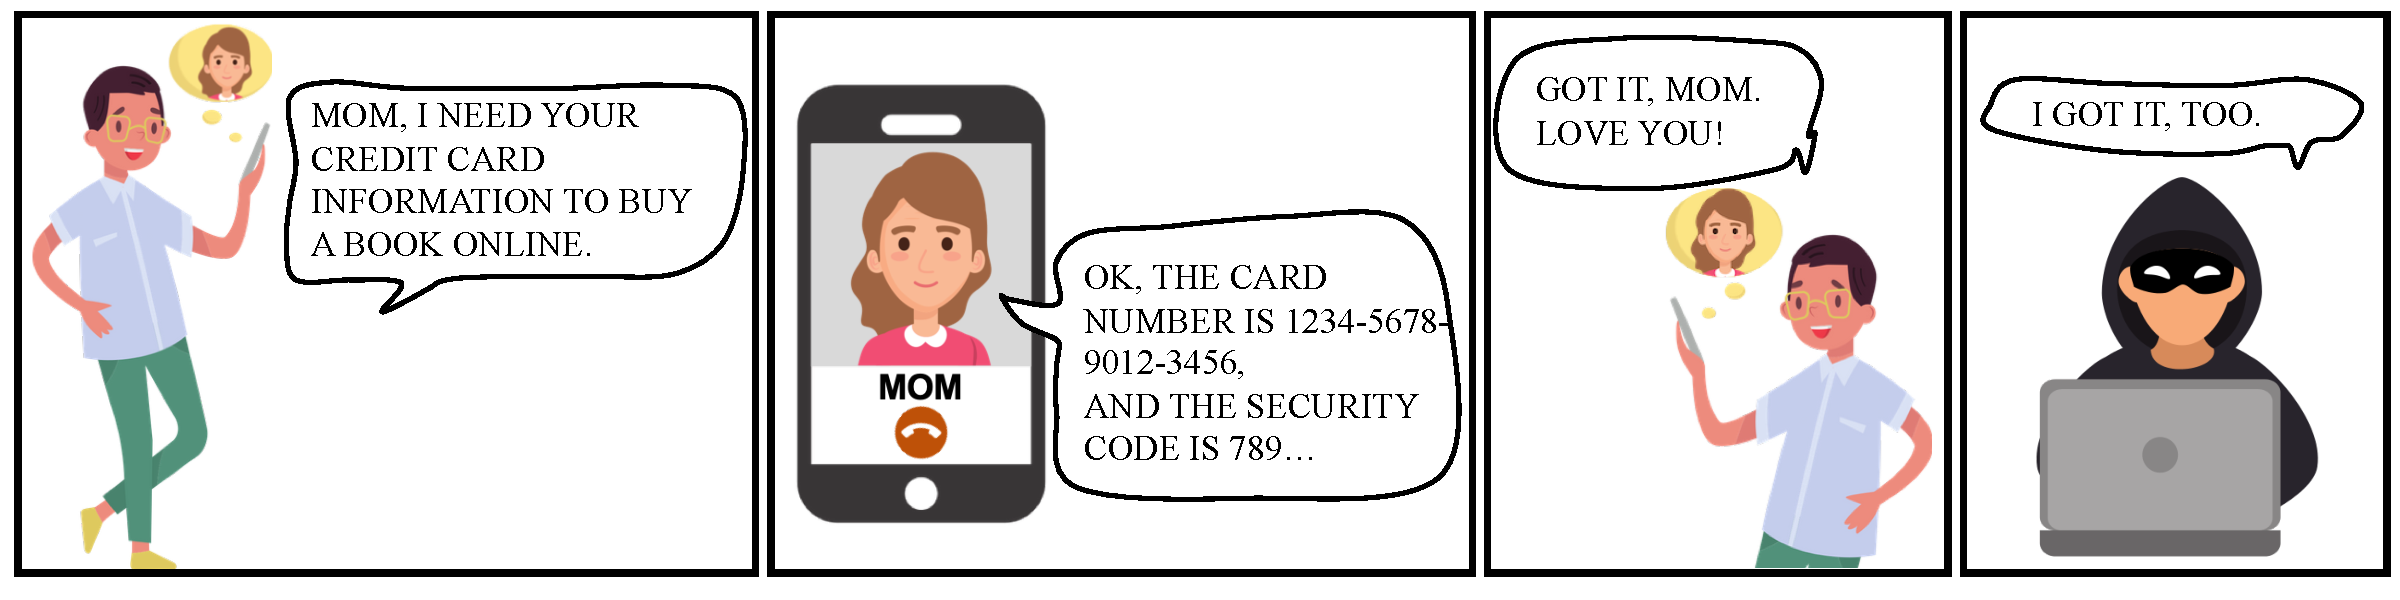
\includegraphics[width=\linewidth]{Figures/SpyPhone/teaserpic}
	\caption[Example of an Attacking Scenario.]{Example of an Attacking Scenario by {\spp}. A seemingly harmless application (a weather app for example) is installed on the phone, and it keeps accessing the motion sensors in background. Attackers can infer acoustic signals from the under-sampled motion data. }
	\label{fig:teaserpic}
\end{figure}



In fact, there have been some recent studies about the side-channel leakage from acoustic signals to smartphones' motion sensor readings. Michalevsky et al.~\cite{michalevsky2014gyrophone} proposed \textit{Gyrophone} in 2014. To the best of our knowledge, they are the first to use smartphone gyroscopes as low-frequency microphones to listen to loudspeakers. Gyrophone can differentiate 11 digits with 65\% accuracy based on a 10 people dataset.
%Michalevsky et al.~\cite{michalevsky2014gyrophone} are the first to use smartphone gyroscopes as low-frequency microphones. 
%However, they only tested their work on a small dataset (10 people) and achieved a digit recognition rate of 65\%. 
One year later, Zhang et al.~\cite{zhang2015accelword} proposed \textit{AccelWord}, which utilizes accelerometers to classify hotwords such as ``Okay Google'' or ``Hi Galaxy'' over other short phrases with 85\% accuracy. AccelWord is also tested over 10 people.
%However, their work lacks credibility due to limited dataset (10 people) and small classifying number (3 classes). 

However, techniques proposed in neither Gyrophone nor AccelWord can be used to perform a {\attackName} attack. Because these systems are built upon a \textit{speaker-dependent} model, i.e. training dataset are labeled data from the target speakers. In the {\attackName} attack, attackers will not get \textit{labeled} motion data from the victim  ------ the attack system should be \textit{speaker-independent}.

In 2018, Anald and Saxena~\cite{anand2018speechless} reproduced the aforementioned works and overturned their conclusions. They argued that smartphone motion sensors can not be affected by the speech signals transmitted through the air, no matter the sound source is a loudspeaker or a live person. They reported that only when the speakers and the motion sensors sharing a surface,  the \textit{conductive vibrations} will affect motion sensors' readings. Except for this ``Loudspeaker-Same-Surface'' scenario, they studied 5 other  scenarios
\footnote{\scriptsize``Loudspeaker-Different-Surface'', ``Laptop-Same-Surface'', `` Phone-Different-Surface'', 		``Human-Normal'', and ``Human-Loud''.}  
%(``Loudspeaker-Different-Surface'', ``Laptop-Same-Surface'', `` Phone-Different-Surface'', 		``Human-Normal'', and ``Human-Loud'')
and concluded that smartphone motion sensors only pose a limited threat to speech privacy.
% since conductive vibrations are ``possibly less common''.
%the impact of speech signals is very limited on motion sensors. 
%
However, they missed one important scenario,  the \textit{intra-device} scenario, where the speakers and motion sensors are inside the same smartphone. In 2019, they investigated this remaining scenario in an arXiv paper~\cite{anand2019spearphone} and their SpearPhone system recognize 11 digits with an accuracy of 71\%.  However, their technique is still speaker-dependent, which means the original speech data of the target speaker must be collected ahead of time. Such requirement is very hard to be fulfilled in practice.

In this thesis, we studied the side-channel attack in the intra-device scenario. This \textit{{\attackName}} attack, as we refer to it, is speaker-independent.


%\begin{figure}[!h]
%\centering
%\subfloat[][]{.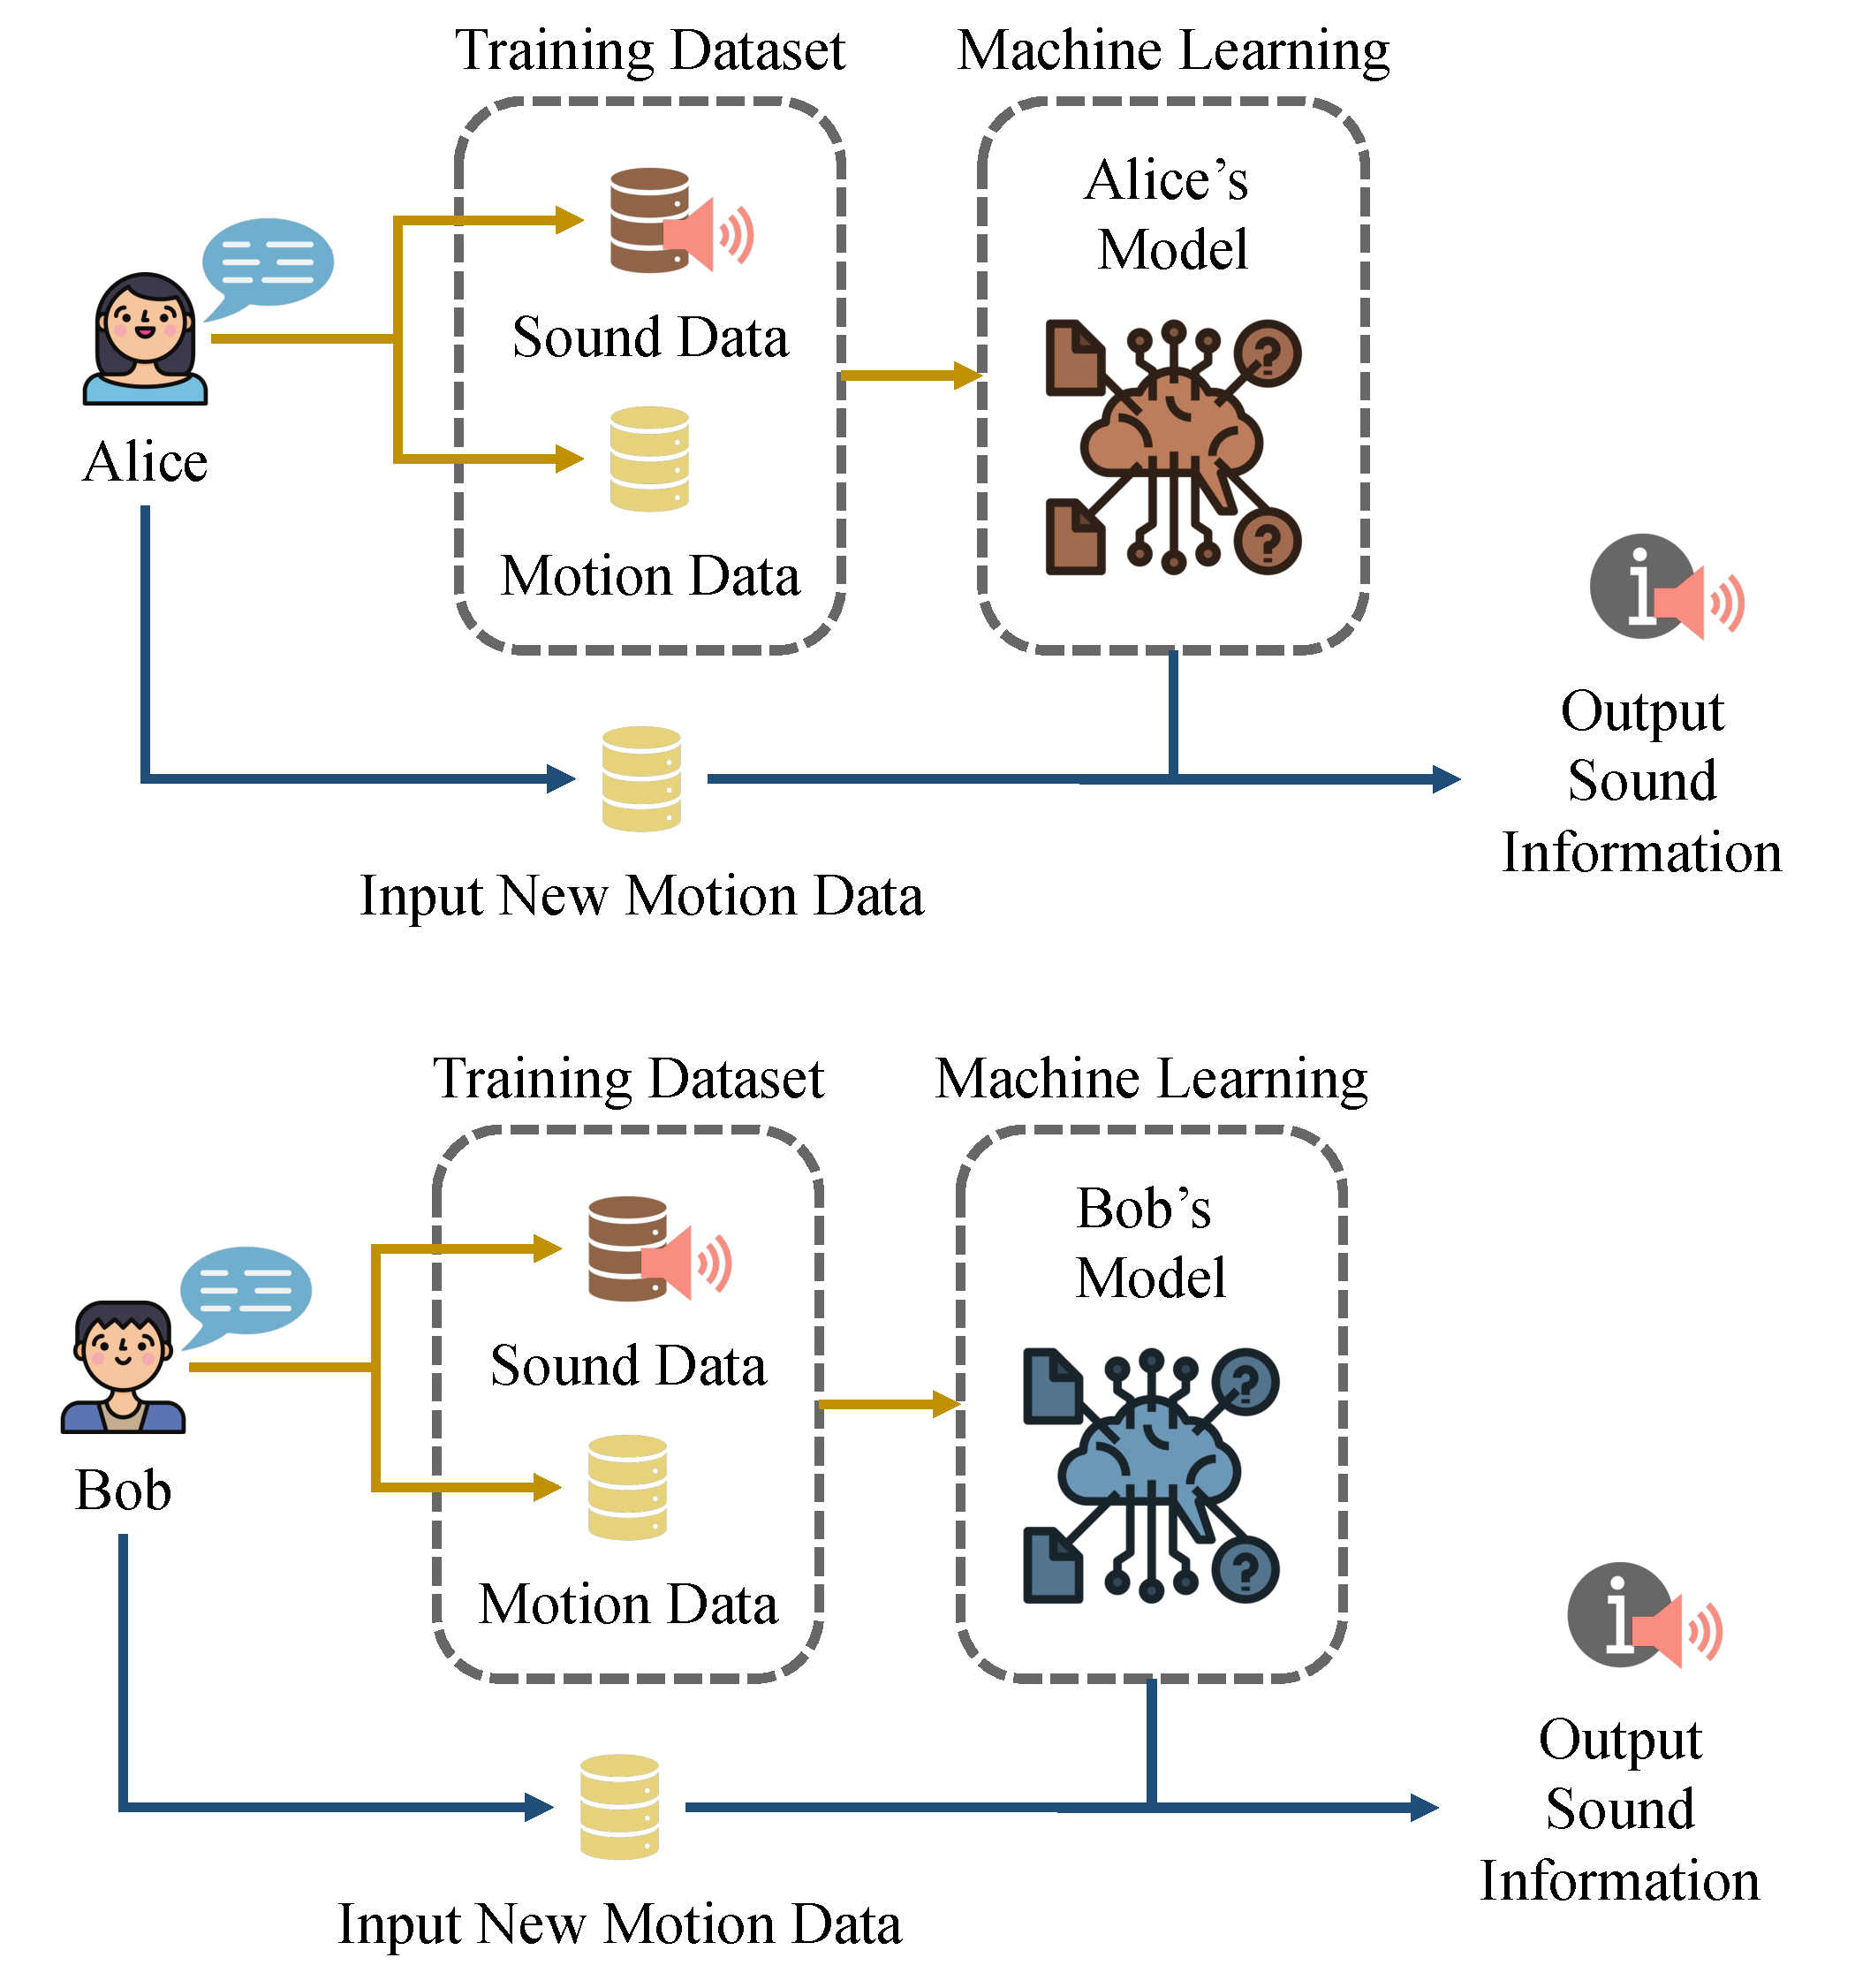
\includegraphics[width=.9\linewidth]{speakerDependent}
%	\vspace{-.05in}
%	\caption{Mathematical model of a typical compressed sensing system. }%
%\qquad
%\subfloat[][]{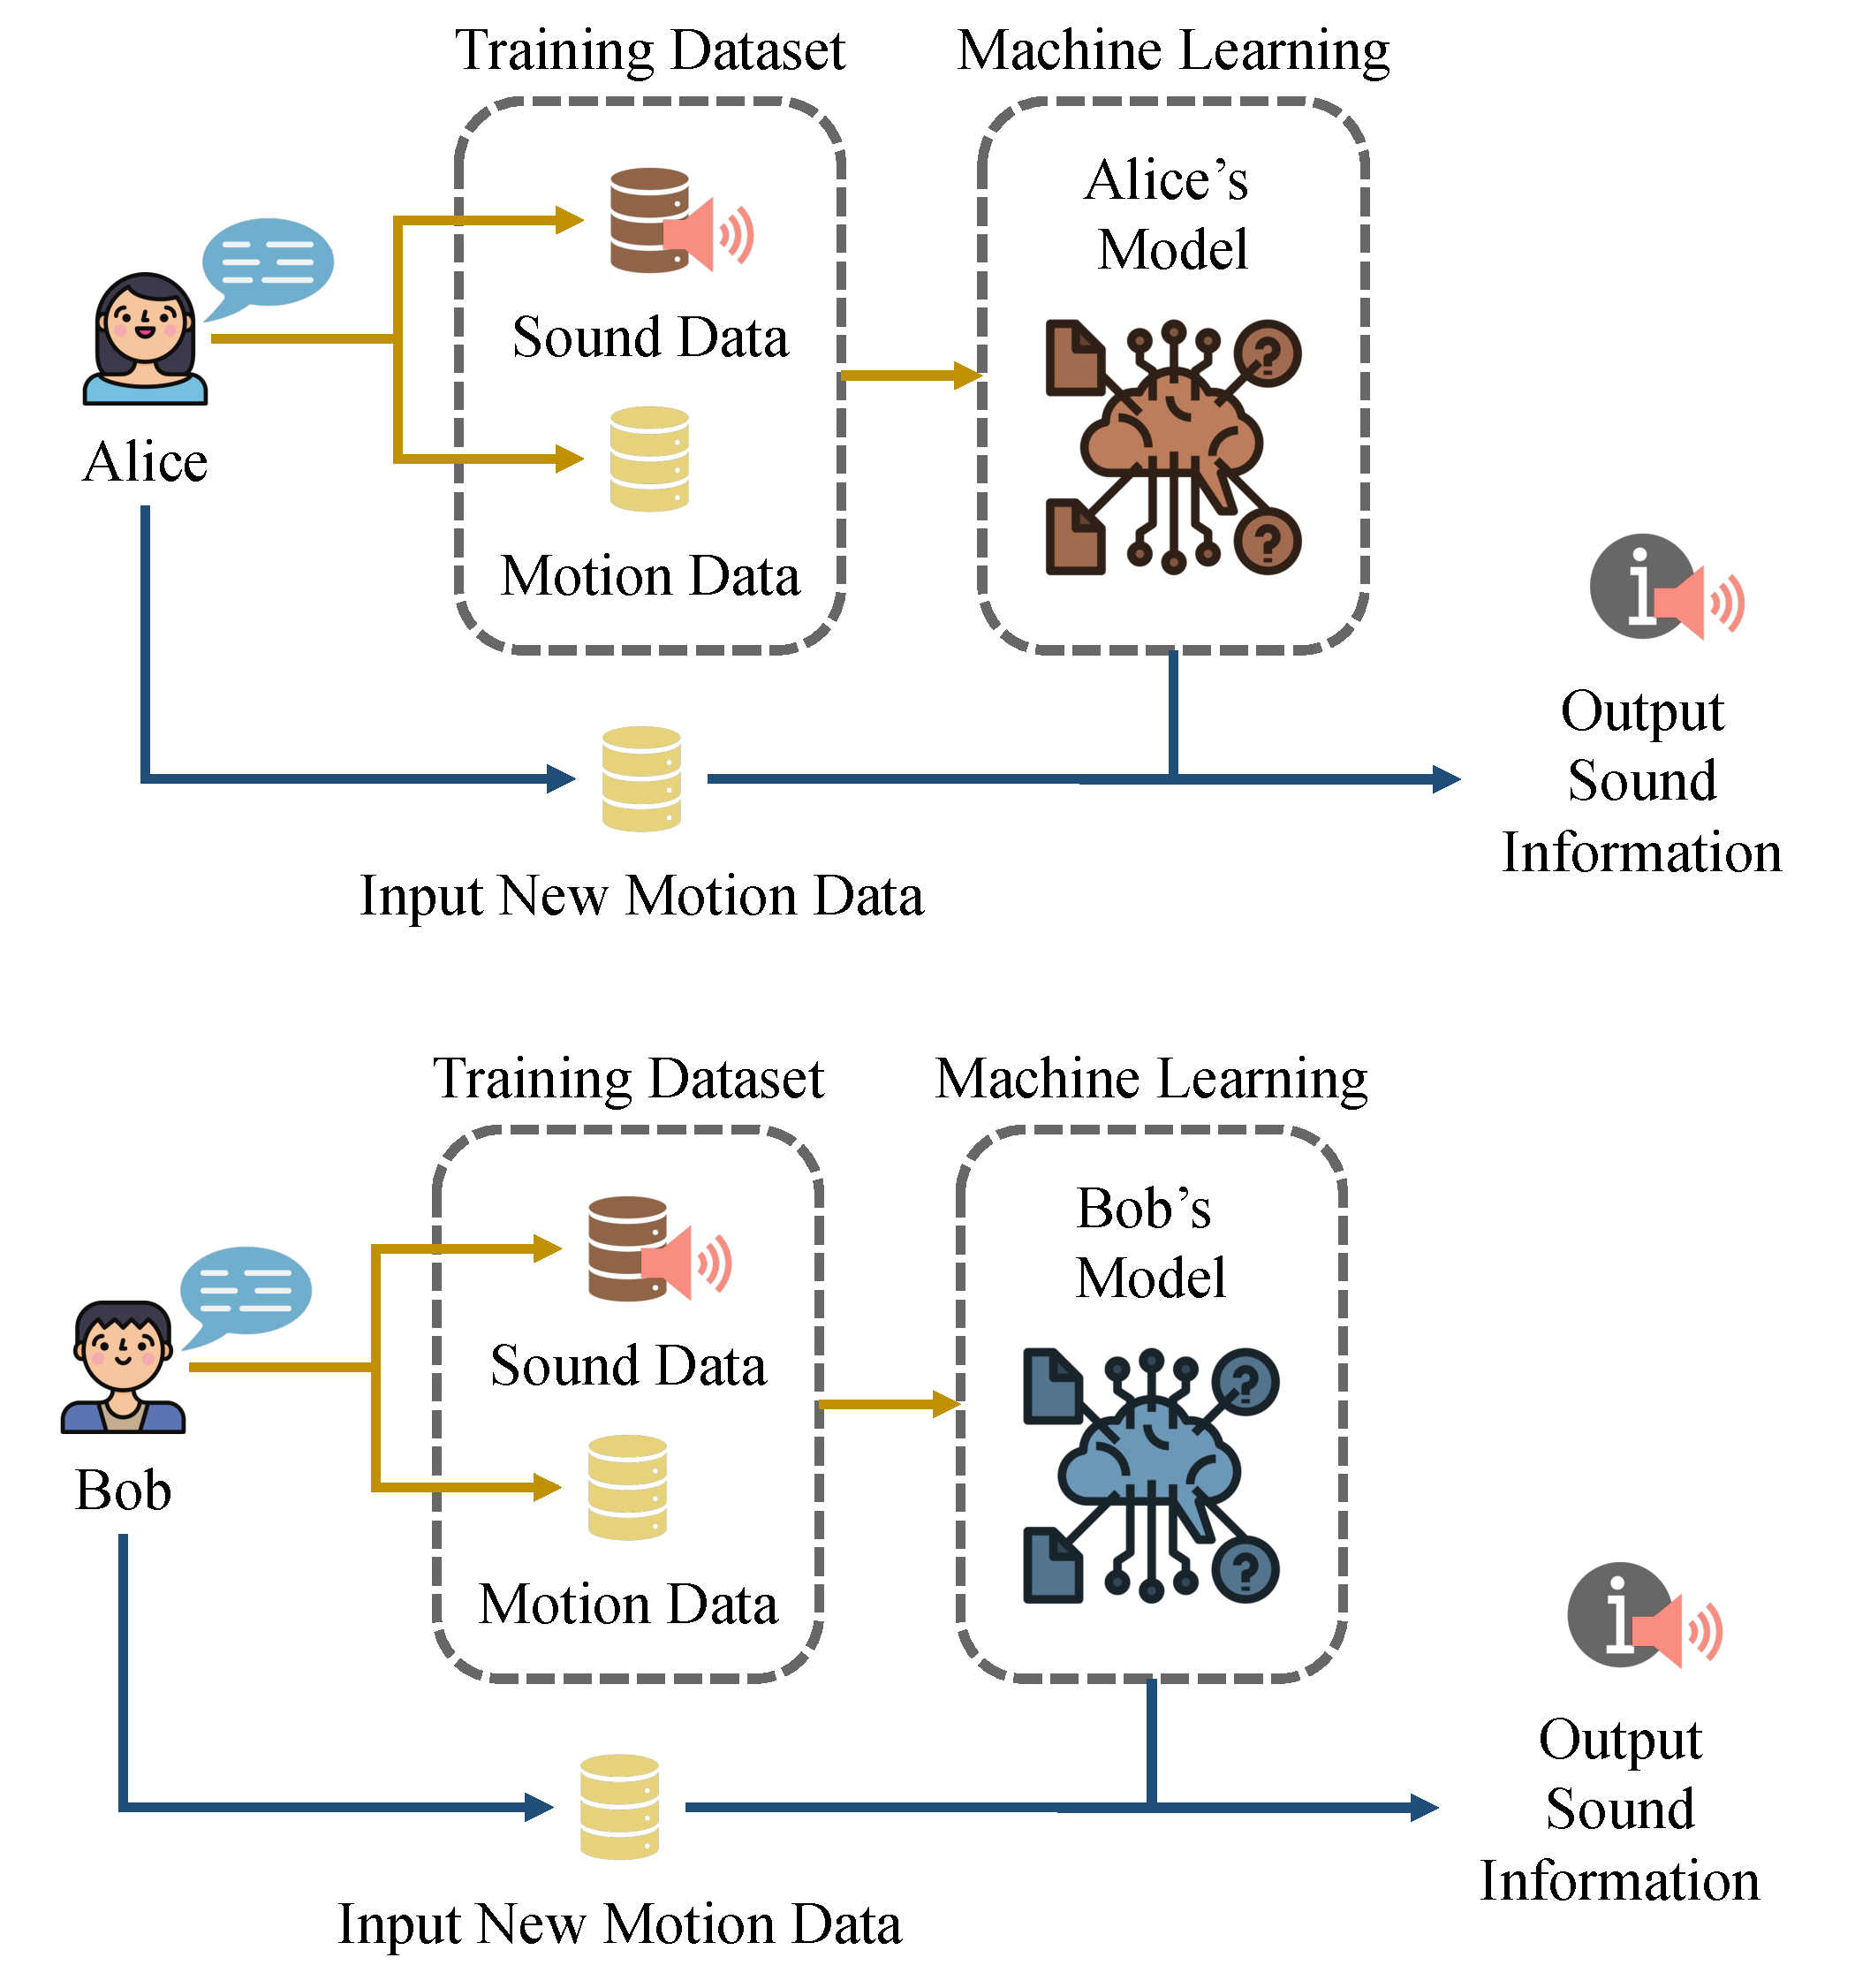
\includegraphics[width=.9\linewidth]{speakerDependent}
%	\vspace{-.05in}
%	\caption{Mathematical model of a typical compressed sensing system. }
%\caption{Here are the first two figures of a continued figure.}% \label{fig:cont}
%\end{figure}
% Attackers do not need to get the target victim's speech data and they can still filch critical information from the 


% https://arxiv.org/abs/1907.05972
%The side-channel attack in this scenario, or the \textit{{\attackName}} attack as we refer to it, is the focus of this paper. We agree with Anald and Saxena on that motion sensors are more sensitive to conductive vibrations than aerial vibrations, but we show motion sensors can leak various critical information and pose a big threat to smartphone users' security and privacy. 

% accelerometer when the laptop and the motion sensor shared a surface.
%
%direct acoustic aerial vibrations 
%
%
%aerial vibrations. We also report that in the presence of live human speech, we did not 
%
% the recorded effect on the sensor readings is possibly from conductive vibrations through the shared surface instead of direct acoustic vibrations due to speech as perceived in previous work. S
%
%
%. They stated that smartphone speakers were not found to be powerful enough to invoke a response in the motion sensors \textit{through aerial vibrations}. They also reported that in the presence of live human speech, they did not notice any effect on the motion sensor readings.

%Different research groups draw conflicting conclusions. So who is right? We have done similar experiments and the findings are similar to that of Anald and Saxena. Unless a person speaks really loudly (shouting, usually 10 dB higher than normal speech),  or use commercial loudspeakers (not MEMS speakers inside smartphones) on the same surface with the smartphone, it is hard to identify the sounding period based on motion sensors. Moreover, the distance between the sound source and the smartphones must be short (less than 30 cm). 

%However, Anald and Saxena's work is not perfect. Although they studied this side-channel leakage in 6 different scenarios and showed the threats only have significant impacts in the ``Loudspeaker-Same-Surface'' scenario, they missed one important scenario, the \textit{intra-device} case, where the speakers and motion sensors are inside the same device. This scenario, or the \textit{{\attackName}} attack as we refer to it, is the focus of our research.

%
%It is also worth mentioning that prior works such as  Gyrophone~\cite{michalevsky2014gyrophone} and AccelWord~\cite{zhang2015accelword} can only achieve the claimed accuracy in the speaker-dependent setting. But a speaker-dependent setting requires the system to get specific training data from the target user. Such condition may not be satisfied in real attacking scenarios. When Gyrophone use an speaker-independent setting to identify digits, the maximum accuracy  is only 26\%.

\begin{table}[h]
	\caption{Maximum Sampling Rate of Smartphone Sensors}
	%	\footnote{Some part of the data is from~\cite{matyunin2018zero}, others are tested }
	\label{tab:sample}
	\centering
	
	%	\resizebox{\columnwidth}{!}{
	\begin{tabular}{cccc} %{lp{2cm}p{2cm}}
		\toprule		
		Device & \makecell{Release \\Year} & \makecell{Speakers' \\ Sampling Rate} & \makecell{Motion Sensors' \\ Sampling Rate
			\footnotemark} \\
		\midrule
		Samsung Galaxy S8 & 2017 & 192,000 Hz & 500 Hz\\
		Samsung Galaxy S7 & 2016 & 192,000 Hz & 500 Hz\\		
		Google Nexus 6P & 2015 & 48,000 Hz & 400 Hz\\
		LG Nexus 4 & 2012 & 48,000 Hz& 200 Hz\\
		\bottomrule
	\end{tabular}
	%}
\end{table}



\footnotetext{\scriptsize Data is partially from~\cite{matyunin2018zero} and partially by calling the \texttt{getMinDelay()} function of \texttt{android.hardware.Sensor} class.}

%To sum up, we show how to design an eavesdropping system that measures the conductive vibrations from smartphones' built-in MEMS speakers to MEMS accelerometers and gyroscopes. The main challenges in performing such an attack are:
%In this paper, we design an eavesdropping system named \textit{{\systemName}} which implements the speaker-independent {\attackName} attack. 
The main challenges in designing such a system are:
 \begin{itemize}
 	\item  The motion sensor readings are affected by at least four types of signal sources: sensor intrinsic errors, movement of the smartphone, acoustic vibrations from built-in speakers, acoustic vibrations from the air or other sound sources. An efficient filter is needed since only the acoustic vibrations from built-in speakers is the signal of interest.
 	
 	\item As shown in Table~\ref{tab:sample}, compared to the sampling rate of smartphones' built-in speakers which can reach 192 kHz, the sampling rate of motion sensors is 200-500 Hz. With such low frequency, human ears are no longer able to retrieve the original information, neither do state-of-the-art speech recognition systems~\cite{michalevsky2014gyrophone}.
 	
 	\item As illustrated in Figure~\ref{fig:depend}, the system should be speaker-independent. Prior works such as  Gyrophone~\cite{michalevsky2014gyrophone} and AccelWord~\cite{zhang2015accelword} can only achieve the claimed accuracy (65\% for 11 classes and 85\% for 3 classes) in the speaker-dependent setting. When Gyrophone uses an speaker-independent setting to identify digits, the
 	accuracy is only 26\%. This indicates that building a speaker-independent system is much more challenging than a speaker-dependent one.
 	
% 	harder than a speaker-dependent system.
% 	%TODO.
% 	In addition
% 	However, the speaker-dependent setting requires the system to get specific training data from the target user. Such condition may not be satisfied in real attacking scenarios. 
 \end{itemize}

%
%44.1 kHZ, 48kHz, 96kHz, or even 192kHz\footnote{Example sampling rate as shown in \url{https://developer.android.com/ndk/guides/audio/sampling-audio}.}, 
%The impact of the studied threat under the designed scenarios therefore limits itself to only specific settings. F
%
%
%information leakage from physical properties, or side-channels


%
%Consequences:
%know the gender
%know the number
%know your activity
%
%Contributions
%

%How we conquer the challenges?

%Although reconstructing original sound signals from motion data is impossible, partial information can be learned by {\attackName} attackers. Such information includes user activity, speaker gender/identity, and speech content (as elaborated in Section~\ref{sec:threat}). 

%\footnote{We refer the attack as the {\attackName} attack, and the system designed to perform such an attack as the {\systemName} system.}



Despite these challenges, the {\systemName} system is able to learn variety of critical information from smartphone users, such as user activity, speaker gender/identity, and speech content (as elaborated in Section~\ref{sec:threat}). 
These achievements are largely credited to the compressed sensing theories which allow recovering certain signals from fewer samples than required in Nyquist paradigm (as elaborated in Section~\ref{sec:background}); and the machine learning techniques named Bi-directional Long Short-Term Memory (Bi-LSTM) network, which is a special variant of recurrent neural networks. 




\begin{landscape}
	\begin{figure*}[h]%
		\centering
		\begin{minipage}[c]{.45\linewidth}
%			\begin{subfigure}[t]{1.3\textwidth}
				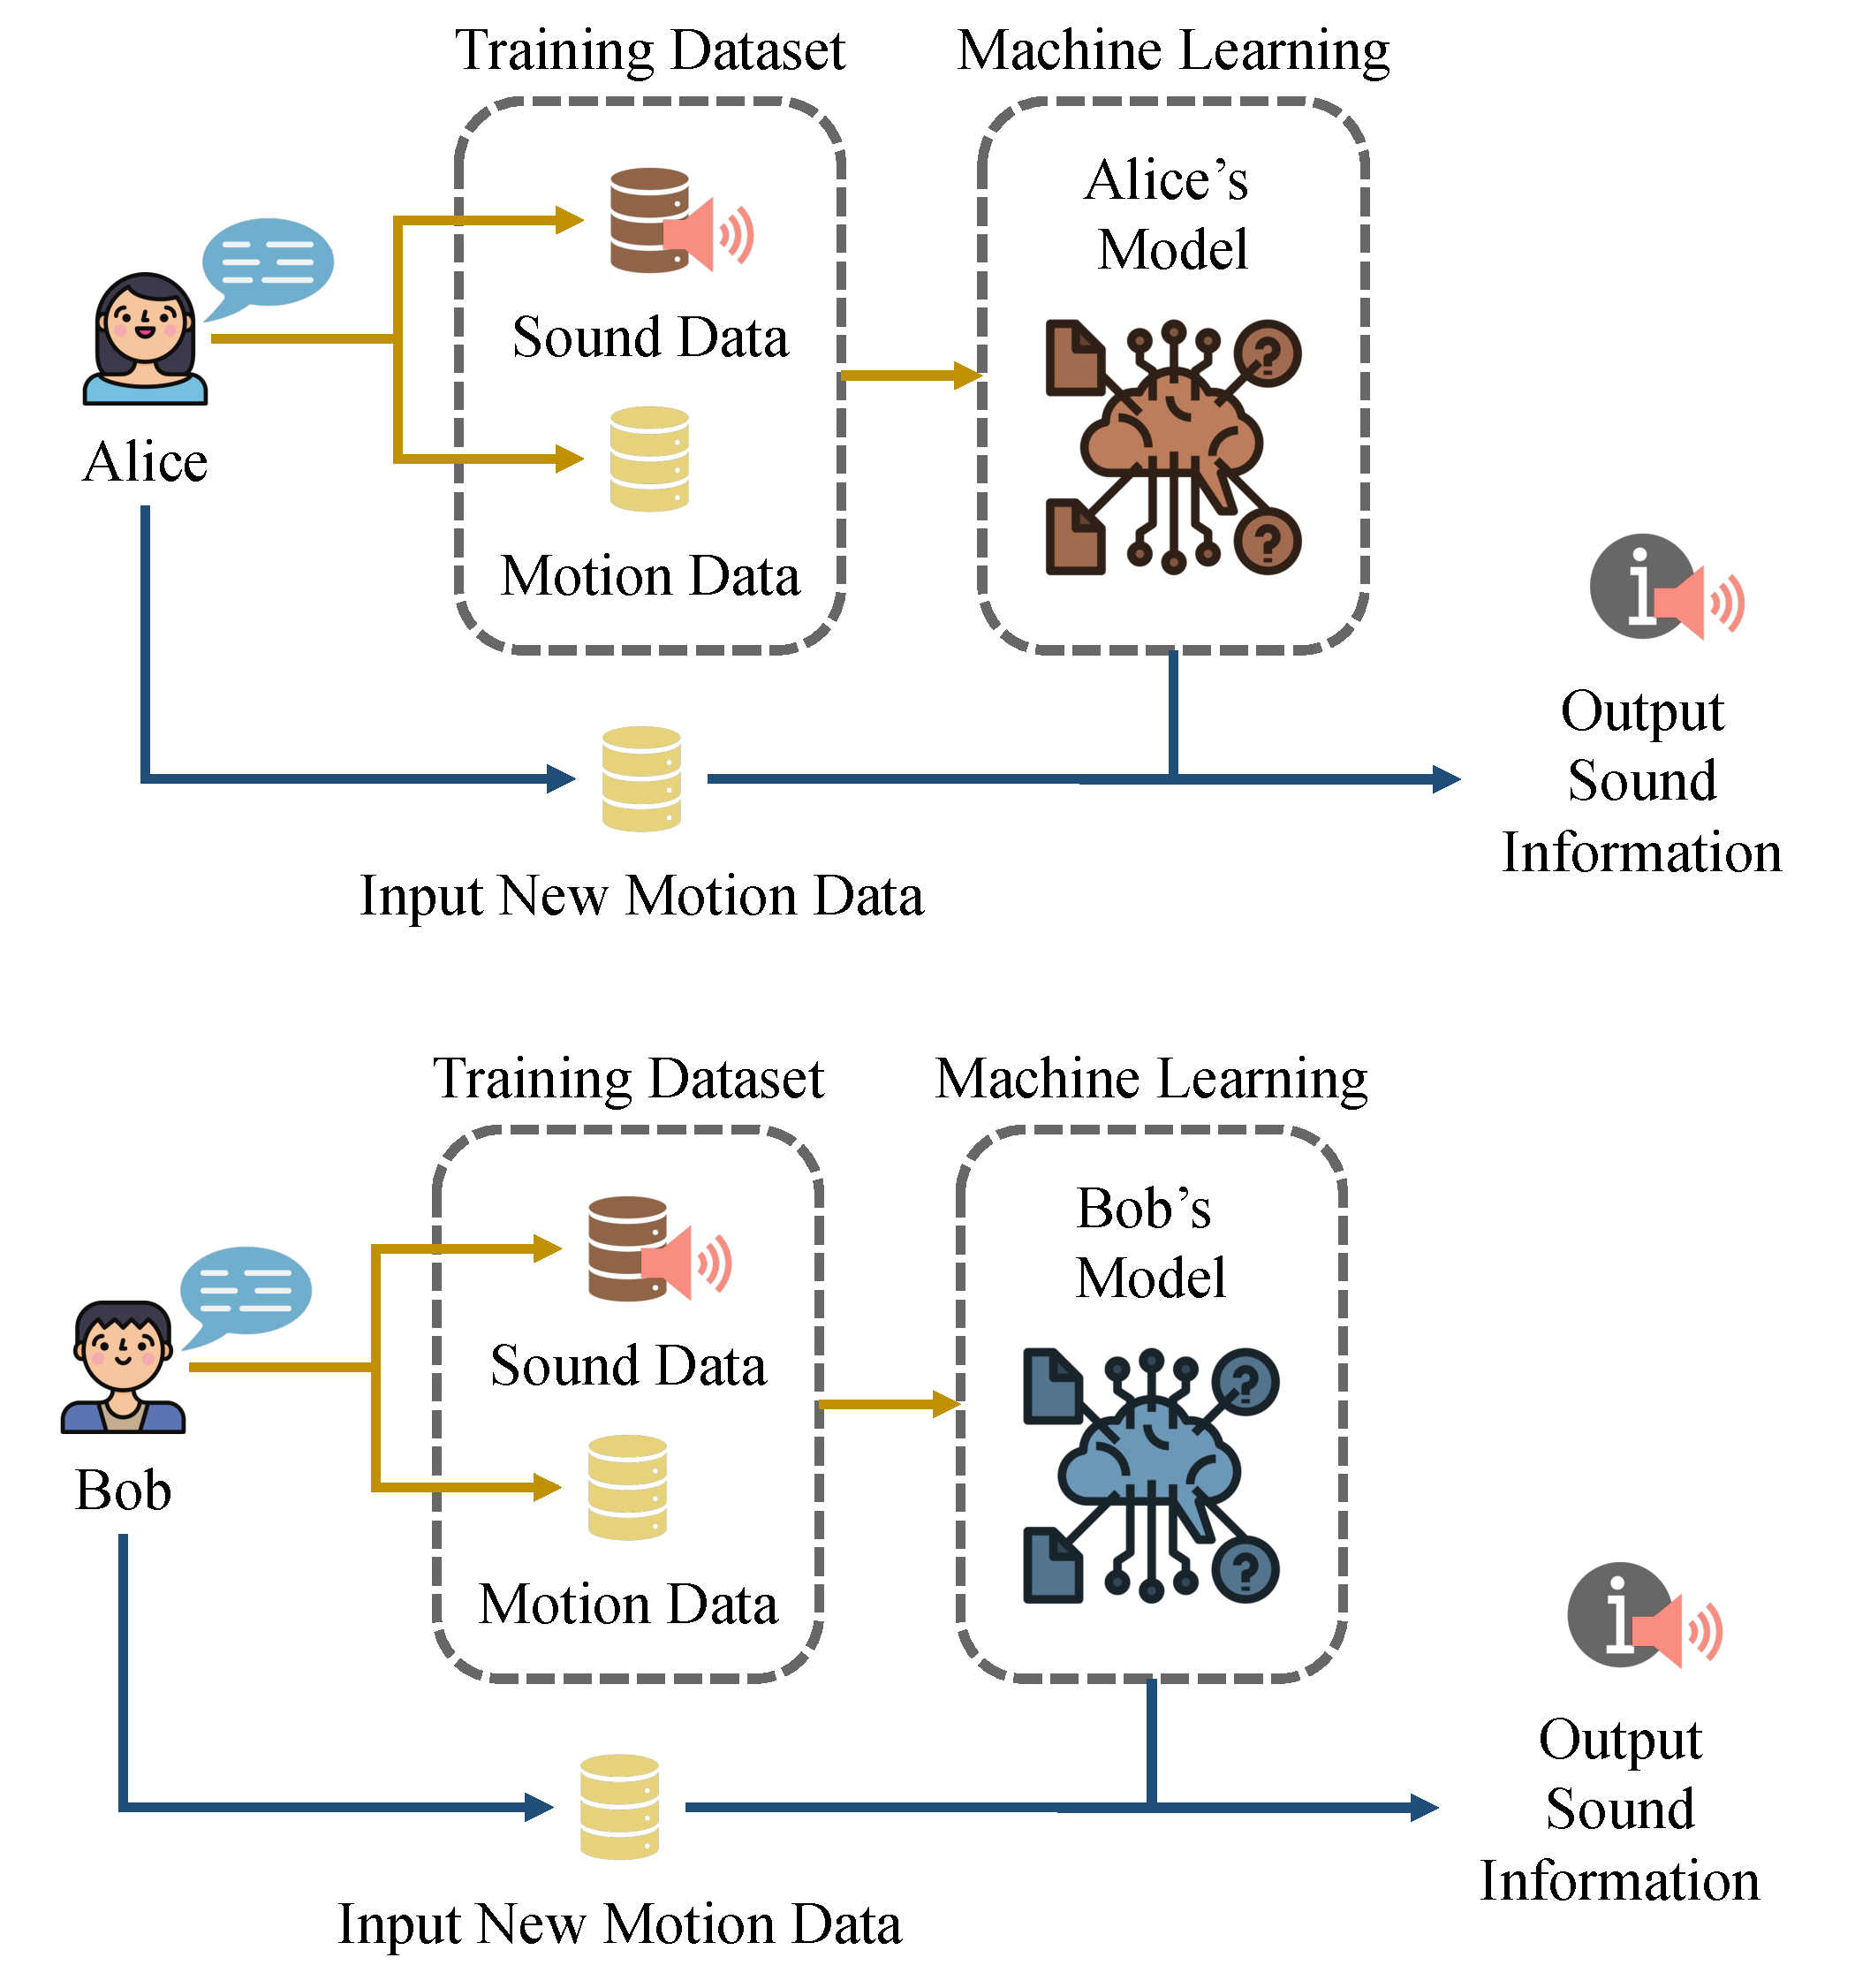
\includegraphics[width=\textwidth]{speakerDependent}
				\subcaption{Speaker-Dependent: target speaker's training data is required. After machine learning procedures, the trained models  for different speakers are different.}
%			\end{subfigure}
		\end{minipage}
		\begin{minipage}[t]{.05\textwidth}
			\qquad
		\end{minipage}
		\begin{minipage}[c]{.45\linewidth}
%			\begin{subfigure}[t]{1.25\textwidth}
				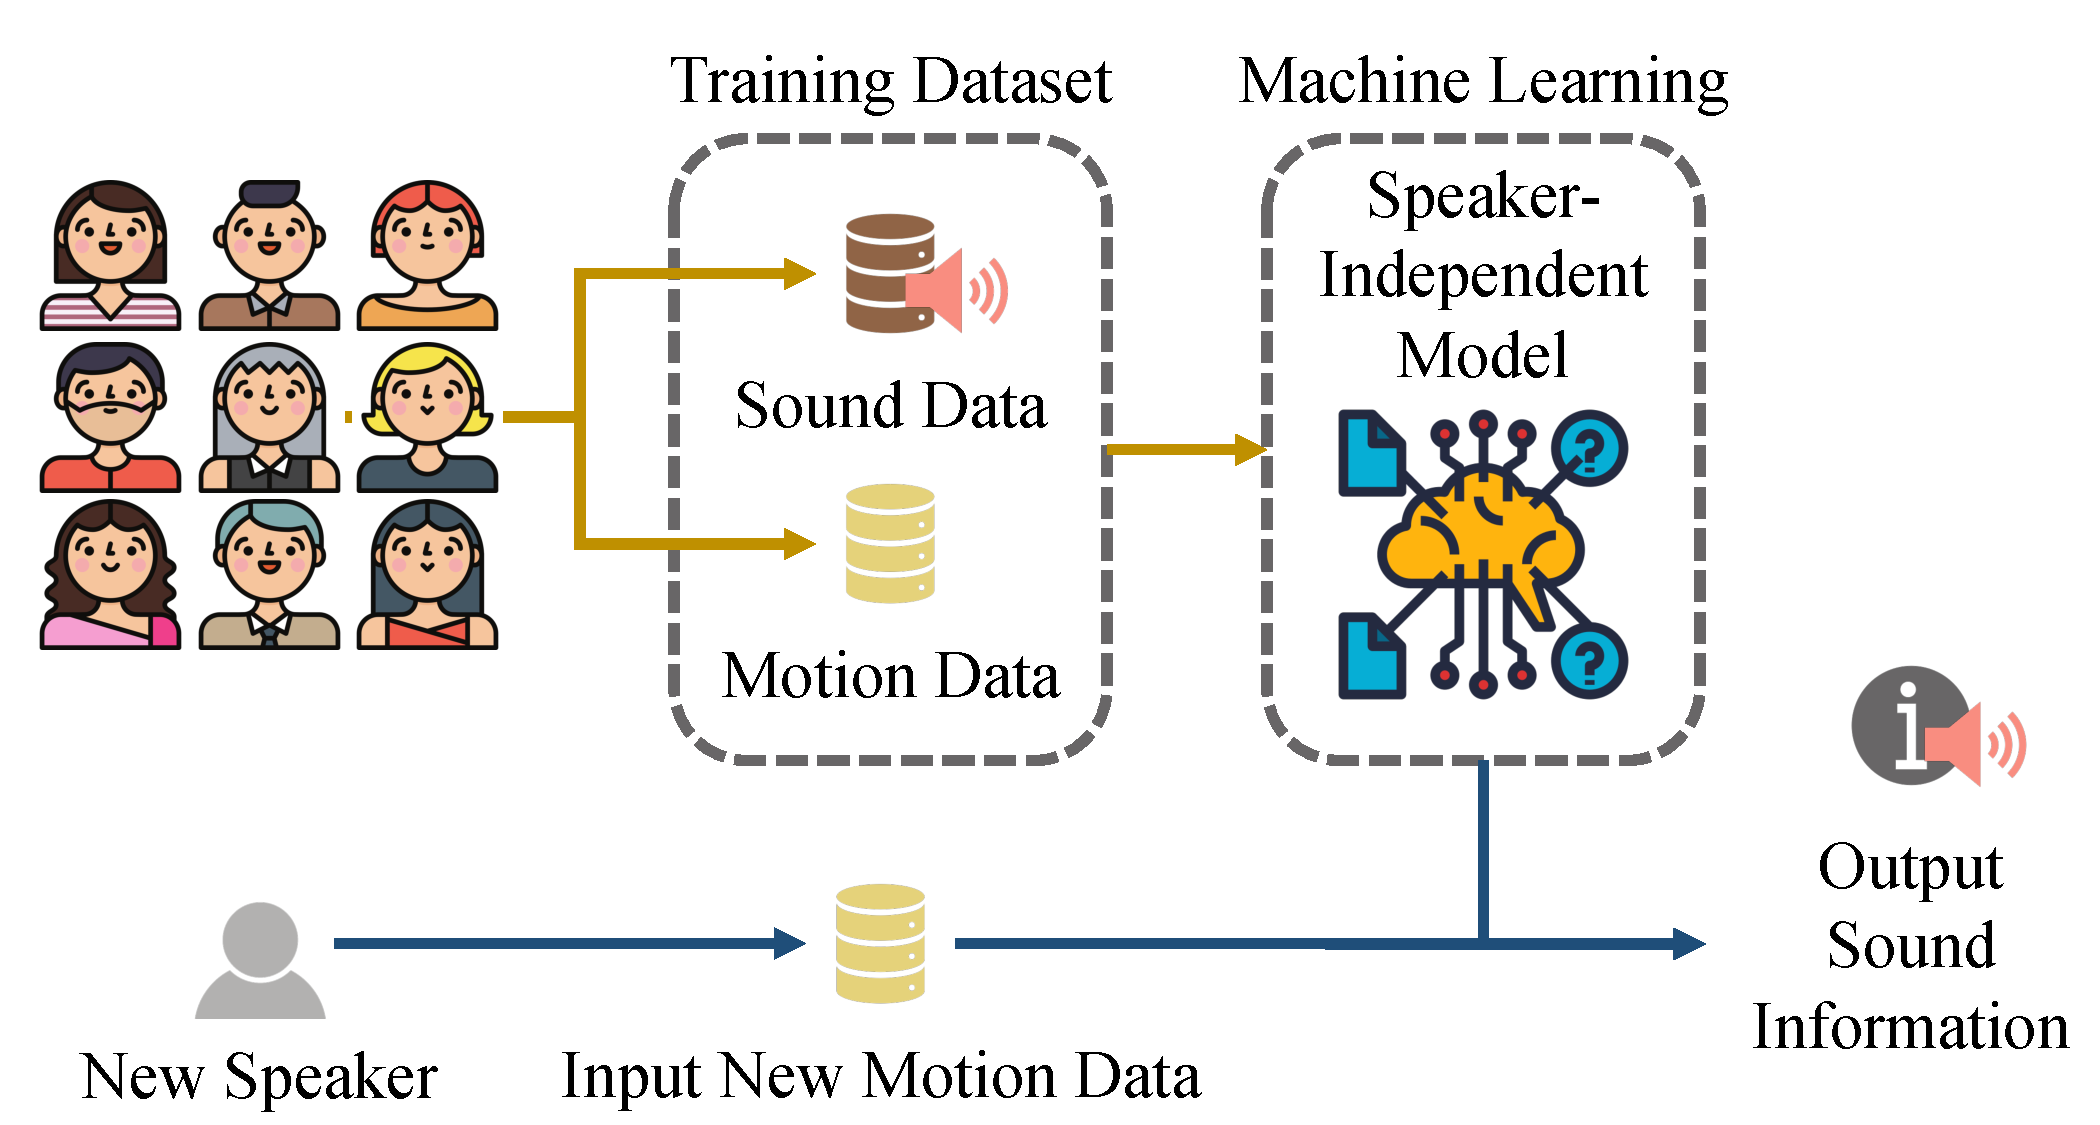
\includegraphics[width=\textwidth]{speakerIndependent}
				\subcaption{Speaker-Independent: the model is trained on a group of speakers, and can be used to predict brand new speakers.}
%			\end{subfigure}
		\end{minipage}
		\caption{{\attackName} Attack Should be Speaker-Independent.} \label{fig:depend}
	\end{figure*}
\end{landscape}

%We conquer the challenges by various  signal processing techniques 

%In summary, our contributions are listed as follows.
%This dissertation offers the following contributions:
%The main contributions are summarized as follows:
%
In summary, our main contributions are as follows:
\begin{itemize}
	\item 
	We uncover a new stealth attack named the {\attackName} attack that eavesdrops on smartphones' built-in speakers by the intra-device motion sensors. Existing techniques in Gyrophone~\cite{michalevsky2014gyrophone} and AccelWord~\cite{zhang2015accelword} cannot be used for the {\attackName}  attack because their system are speaker-dependent, which require the training speech data from the victim. The {\attackName}  attack, however, removes this requirement and thus is more dangerous and harmful.
	
	\item 
	To the best of our knowledge, we are the first to apply compressed sensing theories in the audio-to-motion side-channel data so as to bridge the gap between sampling rates. This is the core technique we used to achieve speaker-independent of the attacking system.
	
	
	\item 
	We design the {\systemName} system and validate its feasibility on learning user activity, speaker gender/identity, and speech content.  {\systemName} system can achieve higher accuracy than existing works. In addition, we have studied how different internal parameters (used in algorithms) and external parameters (properties of input data) affect the  performance of this system.
	
	
%	\item User-independent no individual training
%	
%	Unnoticeable, universal
\end{itemize}


















%%%%%%%%%%%%%%Materials%%%%%%%%%%%%%%



%~\cite{aaaGoogleSearch,michalevsky2014gyrophone,matyunin2018zero}

%
%Any app installed on a smartphone  is permitted to access to motion sensors 


%the system automatically grants the app that permission at install time. 
%%TODO side channal attack??

 
%Why can smartphones provide so many efficient and user-friendly applications? Because these smart devices seamlessly integrate the physical world with the cyber world via their sensors (e.g., light, accelerometer, gyroscope, microphone, speaker, camera, GPS, etc.)~\cite{sikder20176thsense}.
%
%
%
%However, the presence of sensors also has the dark side: \textit{sensor-based attack}s on smartphones. 
%
%The feasibility of keystroke inference from nearby key- boards using accelerometers has been shown in [35]. In [21], the authors demonstrate the possibility of keystroke inference on a mobile device using accelerometers and mention the potential of using gyroscope measurements as well, while another study [19] points to the benefits of exploiting the gyroscope.
%While the number of applications using different sen- sors [38] is increasing and new devices offer more sen- sors, the presence of sensors have opened novel ways to exploit the smart devices [76]. Attackers can exploit the sensors in many different ways [76]: they can trig- ger an existing malware on a device with a simple flash- light [28]; they can use a sensor (e.g., light sensor) to leak sensitive information; using motion sensors such as ac- celerometer, and gyroscope, attackers can record or steal sensitive information from other nearby devices (e.g., computers, keyboards) or people [10, 87, 26, 42]. They can even transfer a specific malware using sensors as a communication channel [76]. Such sensor-based threats become more serious with the rapid growth of Apps uti- lizing many sensors [6, 2].
%
%
%In fact, these sensor-based threats highlight the flaws of existing sensor management systems used by smart devices. Specifically, Android sensor management sys- tem relies on permission-based access control, which considers only a few sensors (i.e., microphone, camera, and GPS)1. Android asks for access permission (i.e., with a list of permissions) only while an App is being installed for the first time. Once this permission is granted, the user has no control over how the listed sensors and other sensors (not listed) will be used by the specific App. Moreover, using some sensors is not considered as a vi- olation of security and privacy in Android. For instance, any App is permitted to access to motion sensors by just accessing the sensor API. Access to motion sensors is not controlled in Android.


%Android sensor management
%
%In this paper, we show how to use only motion sensors to eavesdrop on everything played by the smartphones' built-in speakers, i.e., how to turn the existing over 3 billion smartphones to billions of spy-phones.
%
%This attack is based on the fact that...


%Four  papers: Gyrophone, WALNUT, AccelWord, Speechless
%
%
%
%spy bugs and listening devices
%
%Smartphones are everywhere. 
%
%
%
%
%Existing Eavesdropping on smartphones
%
%Prior work like gyrophone and accelword


% Smartphones are everywhere.
%
%versatile handheld devices have become indispensable tools,
%
%Generally, older "feature" phones are capable of voice calls, text messages and the occasional photo, but not much else. Smart phones, on the other hand, are essentially handheld computers. Users can check their email, browse the web, post updates to social media sites, play games, listen to music, watch movies and even shoot video.
%
%The capabilities are so extensive, 
%
%
%From teenagers to seniors, people 
%
%
%However, the ubiquity of smartphones not only bring convenience to legitimate users, but also build a hotbed of new types of attacks.
%
%According to reports issued by several market-research firms,  including Forrester Research, the total number of smartphone users worldwide will reach 3 billion this year—40 percent of the human population. 
%
%Who doesn’t own a Smartphone? Right from teenagers to senior citizens and from businesspersons to business leaders, Smartphone ownership is Ubiquitous and all pervasive. Indeed, it is estimated that nearly 80\% of the world’s population is now connected to each other through the mobile phones with Smartphones constituting the majority of such devices.
%
%
%
%THE dawn of the planet of the smartphones came in January 2007, when Steve ... The smartphone is ubiquitous, addictive and transformative .
%
%
%The Smartphone is everywhere. Its Ubiquity has resulted in new forms of capitalism with Entrepreneurs and Traders using it for direct communication and  ...
%
%
%According to reports issued by several market-research firms, including Forrester Research, the total number of smartphone users worldwide will reach 3 billion this year—40 percent of the human population. For many, these versatile handheld devices have become indispensable tools, providing connections to loved ones, entertainment, business applications, shopping opportunities, windows into the greater world of social media, news, history, education, and more. And of course, they can always be put to use for a quick selfie. With so many devices in so many hands now, the visual landscape has changed greatly, making it a rare event to find oneself in a group of people anywhere in the world and not see at least one of them using a phone. Collected here: a look at that smartphone landscape, and some of the stories of the phones’ owners.

%
\section{Background}

\subsection{Voice Acoustics}\label{sec:voice}

The generation of human voice follows a source-filter model~\cite{fant1960acoustic}. A speech signal can be seen as a source signal (the glottal source at the larynx, or noise generated at a constriction in the vocal tract), filtered with the resonances in the cavities of the vocal tract (tongue, teeth, lips, velum etc. modifying the sound spectrum over time). This theory has been verified using 3-D printed models of two configurations of a vocal tract to generate sounds to generate the vowels in the words ``had'' and ``heard''~\cite{wolfe2016experimentally}. 

%TODO choose one
%The fundamental frequency for speech ($f_0$) is typically 80 to 250 Hz.
A typical adult male will have a fundamental frequency  ($f_0$) of from 85 to 155 Hz, and that of a typical adult female from 165 to 255 Hz~\cite{baken1987clinical,titze1994principles}. The frequencies of the first, second and $i$-th resonances are labeled as  $R_1, R_2, \ldots R_i$, and those of the spectral peaks produced by these resonances are called formants, $F_1, F_2, \ldots F_i $~\cite{titze2015toward}. 

According to~\cite{ladefoged2014course}, English vowels are perceived largely according to the values of the formants $F_1$ and $F_2$. The range of $F_1$ is roughly from 270 to 860 Hz, and that of $F_2$ from 840 to 2790 Hz~\cite{peterson1952control}. As for English consonants, there are six categories: plosive/stop (e.g. /p/), fricative (e.g. /f/), affricate (e.g. /dZ/), nasal (e.g. /m/), lateral (e.g. /l/), and approximant (e.g. /r/). The frequencies of consonants vary a lot. The turbulence of /s/ and /z/ occurs above 3500Hz, and reaches as high as 10,000 Hz, whereas /w/ has $F_1$ from 250 to 450 Hz and $F_2 $ from 600 to 850 Hz~\cite{ladefoged2012vowels}. 

\begin{table*}[h]
	\centering
	\caption[]{Maximum Sampling Rate of Smartphone Sensors}
	%	\footnote{Some part of the data is from~\cite{matyunin2018zero}, others are tested }
	\label{tab:samplerate}
	\begin{tabular}{lccc} %{lp{2cm}p{2cm}}
		\toprule		
				\multirow{2}{3cm}{Device}& \multirow{2}{2.5cm}{Release Year } & Microphones'  & Motion Sensors'  \\
	& & Sampling Rate & Sampling Rate\footnotemark \\
		\midrule
		Samsung Galaxy S8 & 2017 & 192,000 Hz & 500 Hz\\
		Samsung Galaxy S7 & 2016 & 192,000 Hz & 500 Hz\\		
		Google Nexus 6P & 2015 & 48,000 Hz & 400 Hz\\
		LG Nexus 4 & 2012 & 48,000 Hz& 200 Hz\\
		\bottomrule
	\end{tabular}
\end{table*}
\footnotetext{Data is partially from~\cite{matyunin2018zero} and partially by calling the \texttt{getMinDelay()} function of \texttt{android.hardware.Sensor} class. In fact, the sensors can sample at a higher rate, but the operating systems restrict this rate in order to save power or for security concerns. For example, Google Nexus 6P uses Bosch BMI160, whose sampling rate can be 1600 Hz., but Android operating system only supports up to 400 Hz on the phone.}


By Nyquist–Shannon sampling theorem, to properly sample a signal contains no frequency components higher than $f$ Hz, the sampling rate must be at least $2f$ Hz (Nyquist rate). In other words, a sampling rate of 400 Hz (motion sensors' rate of Google Nexus 6P as shown in Table~\ref{tab:samplerate}) can only handle signals whose component frequencies are below 200 Hz. Except for part of the fundamentals, all $F_1$ and $F_2$ frequencies can not be sensed. Therefore, it is impossible to perceive the signals with such a low sampling rate.

Fortunately, the objective of using motion data in {\shortname} is liveness detection and user identification, not signal recovery. With some proper machine learning technology, the undersampled data is informative enough to fulfill the purpose. The reason is, in signal processing, there exists the aliasing phenomenon that high frequency data will have aliases at the low frequency range, which indicates that the information is kept, though distorted.

%Fortunately, thanks to the aliasing  phenomenon and self demodulation effect, the undersampled motion data still contains partial information, which can be used for liveness detection and user authentication .


%\subsection{Aliasing}
%Aliasing is a phenomenon that causes different signals to become indistinguishable (or aliases of one another) when sampled. For a sinusoid of frequency $f$ , sampled with frequency $f_s$, the resulting samples are indistinguishable from those of another sinusoid of frequency $\mid f − N \cdot f_s\mid$ , for any integer $N$. 
%
%Aliasing is an effect that causes different signals to become indistinguishable from each other during sampling. Aliasing is characterized by the altering of output compared to the original signal because resampling or interpolation resulted in a lower resolution in images, a slower frame rate in terms of video or a lower wave resolution in audio. Anti-aliasing filters can be used to correct this problem.


\subsection{Self Demodulation}
Motion sensors not only captures the original sound data, but also captures the modulated signals. In detail, with self demodulation~\cite{berktay1965possible}, the original sounds self interacts  inside  human body,  resulting in sounds with  lower frequency.

\begin{figure}[h]
	\centering
		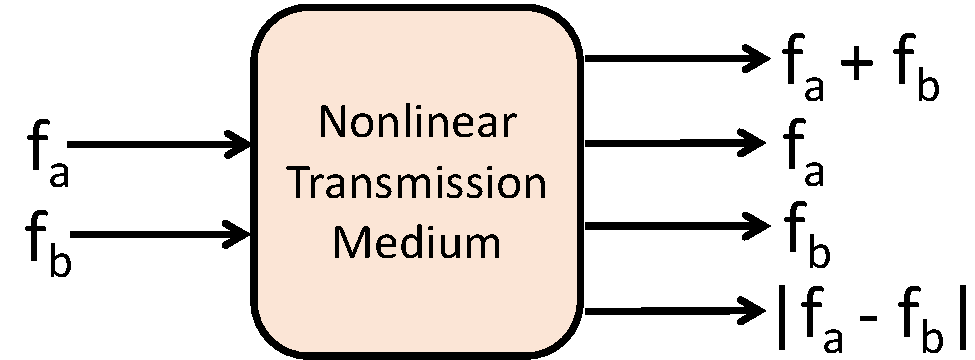
\includegraphics[width=.6\linewidth]{modulation}
	\caption{Self Demodulation of Sound Signals  When Transmitting Through the Human Body.}
	\label{fig:modulation}
\end{figure}

Researchers have found that sounds with different frequencies that transmitted through a nonlinear medium would interact with each other~\cite{pompei1998use}. This interaction produces new frequencies upon the combination of the sums and differences of the individual frequency components by Khokhlov-Zabolotskaya-Kuznetsov(KZK) parabolic nonlinear wave equation~\cite{novikov1987nonlinear}. 

Since the acoustic impedance of the human body is similar to that of water~\cite{kim2014sound}, the self-demodulation would occur in the human body as show in Fig.~\ref{fig:modulation}. 
The original sound signals with frequency $f_a$ and $f_b$ would introduce two more signals with frequency $f_a + f_b$ and $|f_a - f_b|$. For different person, the original signals generated have different frequency, so the low frequency signal $|f_a - f_b|$ are different, which can be utilized for user authetication.
%
Moreover, note that electronic devices has different acoustic property from that of human body. Therefore, those low frequent signals can be used for liveness detection.

%However, borrowing theories from \textit{compressed sensing}, the {\systemName} system can partially reconstruct the signal and obtain critical information such as the numbers appeared in a conversation, genders or even identities of the speakers, etc., from motion sensor readings, as discussed in Section~\ref{sec:threat}.

\subsection{Acoustic Attenuation}
Another effect helps {\shortname} to do spoof-proof authentication is the acoustic attenuation by human body.
%
It is known that human voice is emitted by the vocal organ and is a combination of mechanical vibrations with multiple  amplitudes and different  frequencies.
%
When a person speaks, the  airflow from the lungs through the trachea compresses the vocal cords causing vibrations to make sounds. The lung, trachea and vocal cord form a resonance chamber. 
%\begin{figure}[h]
%	\centering
%		\includegraphics[width=.4\linewidth]{background}
%	\caption{Background}
%	\label{fig:background}
%\end{figure}

Suppose the length of vocal cords is $d$, the lung volume is $V_0$ and the cross-sectional area at the vocal cords is $S$. According to the polytropic process equation, when the airflow moves $d$, the air pressure at the vocal cords can be expressed as follows,
\begin{displaymath}
P_1 = \frac{P_0 \cdot V^\gamma_0 }{(V_0 - d \cdot S)^\gamma},
\end{displaymath}
where $P_0$ is the normal atmospheric pressure, and $\gamma$ is a coefficient about the air specific heat. 
According to the definition of pressure, if the area at the vocal cords is $S_v$,  the force at the vocal cord is,
\begin{displaymath}
F_0 = P_1 \cdot S_v = \frac{S_v \cdot P_0 \cdot V^\gamma_0 }{(V_0 - d \cdot S)^\gamma}.
\end{displaymath}
When the force is applied to the vocal cords, vertical displacement occurs. 
According to the Newton’s second law of motion, we have,
\begin{displaymath}
F(t) = m a(t) + k x(t) + c v(t),
\end{displaymath}
where $F(t)$ is the external force, $v(t)$ is the speed, $x(t)$ is the vertical displacement, $c$ is the damping coefficient, and $k$ is the spring constant and m is the mass. 
The relation can further be explained as,
\begin{equation}
F(t) = m \frac{d^2 x(t)}{d t^2} + k x(t) + c \frac{x(t)}{d t}.
\label{eq:force}
\end{equation}

The vibration during an airflow pass the vocal cords can be separated into two phases. In the first phase, the airflow is passing the vocal cords which is considered to be a forced vibration with constant force $F_0$. After the airflow passed, in the second phase, the pressure of airflow disappears which leaves the system to vibrate on its own and this is called free vibration. In the forced vibration phase, after applying the Fourier transform to both side of e.q.~\eqref{eq:force}, we have,
\begin{displaymath}
\frac{F_0}{j \omega}(1-e^{-j\omega \delta t}) = - \omega^2 m X(\omega) + k X(\omega) + j \omega c X(\omega).
\end{displaymath}
That is,
\begin{displaymath}
X(\omega) = \frac{1-e^{-j\omega \delta t}}{-\frac{j m}{F_0} \omega^3 - \frac{c}{F_0} \omega^2 + \frac{j k}{F_0} \omega},
\end{displaymath}
where $X(\omega)$ is the spectrum of the vertical vibration signal and $\omega$ is the frequency. 
During the horizontal propagation of the vibration signal from the vocal cords to the throat, the vibration suffers from attenuation, and the corresponding model can be stated as follows,
\begin{displaymath}
x_s(t) = x(t) e^{-\alpha d},
\end{displaymath}
where $x_s(t)$ is the vertical displacement at the throat where the vibration has propagated, $x(t)$ is the vertical displacement at the vocal cords, $d$ is the propagation distance, and $\alpha$ is the attenuation coefficient. 
After applying the Fourier transform to both side of e.q.~\eqref{eq:force}, we have,
\begin{displaymath}
X_s(\omega) = X(\omega) e^{-\alpha d}.
\end{displaymath}
Note that $\alpha$ is related to the propagation medium. Wave propagation in body is dispersive by nature, which implies that different frequencies propagate with different attenuation coefficients at different velocities. Roughly speaking, the attenuation is small when the vibration signal propagates through the hard bone, whereas the attenuation is large through the soft tissue. Therefore, vibration waves generated at different positions at throat result in different values of $\alpha$ and $d$, which make the vibration signals unique at different positions. 
After putting all equations together, we obtain,
\begin{displaymath}
X_s(\omega) = \frac{(1-e^{-j\omega \delta t}) e^{-\alpha d}}{(-jm\omega^3 - c \omega^2 + jk\omega)(\frac{(V_0 - d \cdot S)^\gamma}{S_v \cdot P_0 \cdot V^\gamma_0 })}.
\end{displaymath}
For the same location of the human body, $m$, $c$ and $k$ are stable and belong to the same biometric feature. Each person’s lung volume and vocal cords are also different. Therefore, the vibration at the throat of different people can uniquely be identified, which can be leveraged for authentication. The propagation from electronic device to the target smartphone is different from vocal organ through human body. Thus, this effect is also valuable for liveness detection.


%\subsection{Voice Production}
%source-filter model, why our algorithm is user-independent. Similar source, different filter.
%\subsection{Voice Authentication System}
%Attacking (direct/indirect), here we only consider direct.


%



\section{Threat Model in the  {\systemName} System}\label{sec:threat}
%TODO applications

%%TODO
%{attcker vs system}

The attacker's goal is to eavesdrop on everything played by the smartphone speakers  without the user's awareness. 

The attack begins when the user installs a seemingly innocent application, e.g. a car racing game with motion-control steering wheel (tilt the smartphone to steer). 
%
We assume such a disguised app has the access to motion sensors (accelerometers and gyroscopes) as well as the network. This assumption is easy to fulfill since the permissions to motion sensors and the internet are all considered as \textit{normal} permissions by the Android operating system~\footnote{\scriptsize \url{https://developer.android.com/guide/topics/permissions/overview}}. 
%~\cite{onlineoverview}.
In other words, Android automatically grants the app these permissions at installation time. The operating system doesn't prompt the user to grant permissions, and users cannot revoke these permissions. Moreover, almost every smartphone has motion sensors and is able to connect to the Internet. The {\attackName} attack is therefore a threat to every smartphone user.

There is no other requirement for the attacker to conduct a {\attackName} attack. The disguised app just runs in the background and keeps monitoring the motion sensors. Since the power consumption of the motion sensors is very low, the user will not know the motion sensors are in use. In addition, some smartphones are set to be ``Rotation On'' or ``Lift to Unlock", which means the operating system automatically collects motion data, and the {\systemName} system does not introduce extra consumption by using the sensors.

The sensor data are sent back to the attacker over wireless networks. The attacker can choose to transmit data only when the smartphone is connected to Wi-Fi; otherwise, the user may notice the attack through suspicious cellar data usage. The data will be processed at the attacker's end. By utilizing compressed sensing, machine learning and other signal processing techniques, {\systemName} recovers \textit{critical information} from undersampled motion data.
%
The critical information could be, but not limited to,
%\vspace{-.1in}
%, the followings:
\begin{itemize}
	\item
	User activity. Using motion sensor to recognize user activity is not new. However, those activities (e.g., sitting, walking, running or exercising)  are recognized based on different \textit{macro} motions. {\systemName}, on the other hand, is utilizing the \textit{micro} motions caused by speakers. Therefore, {\systemName} can tell whether a user is listening to music or watching an online talk even when the phone seems stationary.Smartphones' built-in speakers are often used for alarms, phone call ringing, music listening, background sound for game playing, and so on. Different activity plays different sound and creates different motion sensor readings. The {\systemName} system can be trained to classify the motion data to these different user activities. Put the matter another way, an attacker can know when the user wakes up, when she receives phone calls, how long she listens to music, or how long she plays games, and so on.
	\item 
	Speaker gender/identity. When the smartphone user has a audio call, video call, or an online meeting with others, the {\attackName} attackers can learn whether the person she talks to is female or male. {\systemName} can also learn how often the user contacts each different person. Moreover, if the attacker could get those people's voice samples (either by recording in public area, or acquiring from social media online, etc.), the attacker can know exactly who they are.
	\item
	Speech content. Another goal for the attacker is to recover the whole speech content by motion sensors. However, considering the tremendous gap between the sampling rate of smartphone speakers and motion sensors, there is still a long way before success. In Section~\ref{sec:design}, as a proof-of-concept, we use digit recognition to demonstrate the design of the {\systemName} system, since the most critical information such as  banking account numbers, credit card information, and certain passwords,  are essentially combinations of digits. In Section~\ref{sec:experiment}, command recognition is also tested.
\end{itemize}

%\vspace{-.1in}
In addition, It is worth mentioning that the {\attackName} attack is built upon a speaker-independent machine learning model and does not require any specific training data from the user. Though with such data, the accuracy might be further improved. Prior works such as Gyrophone~\cite{michalevsky2014gyrophone} and AccelWord~\cite{zhang2015accelword} can only be used in the speaker-dependent case. Using their techniques, the user must obtain the victim's speech first, which is harder to be carried out in reality.

%\begin{itemize}
%	\item User activity. A loudspeaker is commonly used for alarms, phone call ringing, music listening, background sound for game playing, video calling, and so on. Different activity plays different sound and creates different motion sensor readings. {\attackName} system can be trained to classify the motion data to different user activities. Put the matter another way, an attacker can know when the user wakes up, when she receives phone calls, how long she listens to music, or how long she plays games, and so on.
%	\item Speech 
%\end{itemize}


%
%Permissions on sensors
%
%The system doesn't prompt the user to grant normal permissions, and users cannot revoke these permissions.
%
%PatternListener requires the permission to access speaker, microphone, and motion sensors (i.e., accelerometer and gyroscope) as well as network access permission. Most permissions can be granted without user approval, except the permission of accessing the microphone. However, we observe that the permis- sion of accessing microphone is very popular in Android apps. For instance, microphone permissions are required by 55\% social apps and 52\% communication apps in the Google Play marketplace. The details can be found in the appendix. Therefore, it is easy for Pat- ternListener to obtain the permission after it is disguised as an app in these categories.
%
%which ``tilt to steer'', 
%
%motion-control game app.
%
%Meddling with the data occurs using a seemingly innocent application, e.g. a fake flashlight app, within which holds the attacker’s exploit script. 
%We assume the attacker build a 
%
%
%The adversary’s goal is to inject voice commands into the voice controllable systems without owners’ awareness, and execute unauthenticated actions. We assume that adversaries have no direct access to the targeted device, own equipment that transmits acoustic signals, and cannot ask the owner to perform any tasks.
%
%Assumptions
%
%
%Sample rate on Smartphones.
%
%
%No Target Device Access. We assume that an adversary may target at any voice controllable systems of her choices, but she has no direct access to the target devices. She cannot physically touch them, alter the device settings, or install malware. However, we assume that she is fully aware of the characteristics of the target devices. Such knowledge can be gained by first acquiring the device model and then by analyzing the device of the same model before launching attacks.
%No Owner Interaction. We assume that the target devices may be in the owner’s vicinity, but may not be in use and draw no attention (e.g., on the other side of a desk, with screen covered, or in a pocket). In addition, the device may be unattended, which can happen when the owner is temporarily away (e.g., leaving an Amazon Echo in a room). Alternatively, a device may be stolen, and an adversary may try every possible method to unlock the screen. Nevertheless, the adversaries cannot ask owners to perform any operation, such as pressing a button or unlocking the screen.
%Inaudible. Since the goal of an adversary is to inject voice com- mands without being detected, she will use the sounds inaudible to human, i.e., ultrasounds (f > 20 kHz). Note that we did not use high-frequency sounds (18 kHz < f < 20 kHz) because they are still audible to kids.
%Attacking Equipment. We assume that adversaries can acquire both the speakers designed for transmitting ultrasound and com- modity devices for playing audible sounds. An attacking speaker is in the vicinity of the target devices. For instance, she may secretly leave a remote controllable speaker around the victim’s desk or home. Alternatively, she may be carrying a portable speaker while walking by the victim.
%

%
\section{Attack Design}\label{sec:design}


The workflow of the {\attackName} attack in {\systemName} is shown in Figure~\ref{fig:flow}. The system can be separated into two parts: the user side and the attacker side. 
%
On the user side, a smartphone user downloads a seemingly harmless application and installs it on her device. Then the disguised app runs in the background and keeps monitoring the motion sensors. The sensor readings are then uploaded and sent to the attacker. 
%
On the attacker side, there are training steps and prediction steps. The training steps start from a training dataset that contains both sound data and motion data, while the input for prediction steps only contains motion data. 

The training steps first apply compressed sensing techniques on the sound data and build a learned dictionary from audio files, then process the corresponding motion data to remove unwanted signal components. With the preprocessed motion data and a learned dictionary,  the signal is reconstructed to a signal with more samples. Afterward, the reconstructed signal is fed to a Bidirectional Long Short-Term Memory (Bi-LSTM) network to train a classification model. 
The classification labels/classes (e.g. digits, genders, activity types, and so on) is determined by the sound data only.


\begin{landscape}
\begin{figure*}[h]
	\centering
	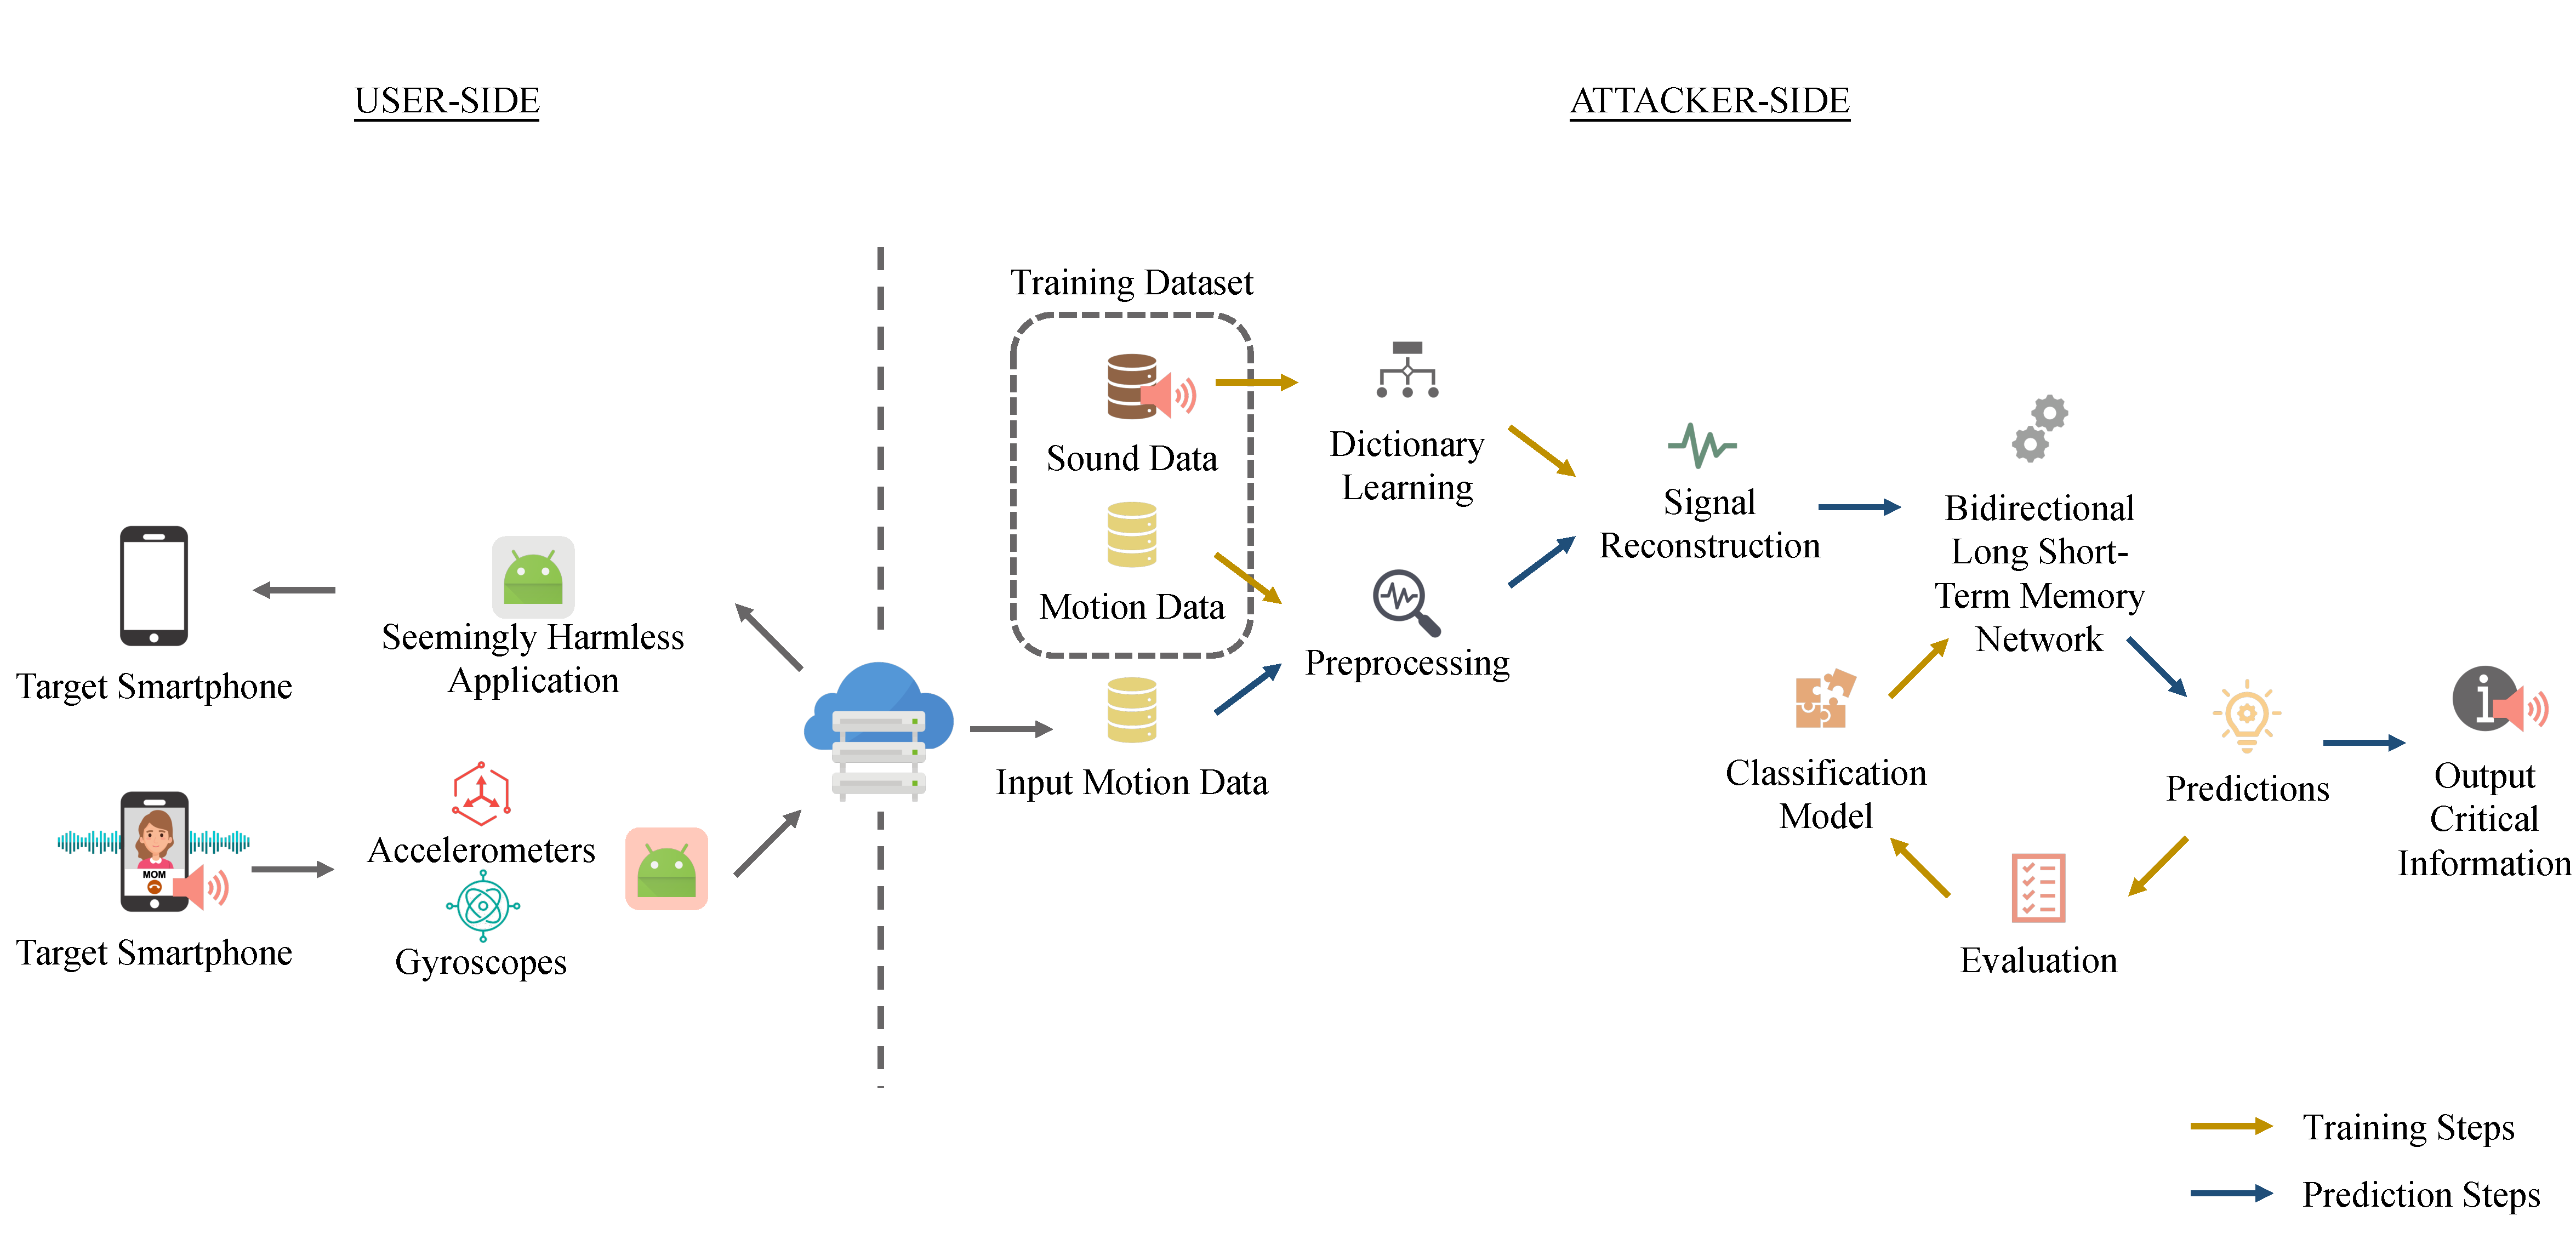
\includegraphics[width=\linewidth]{attackflow}
	\caption{The {\attackName} Attack Workflow in the {\systemName} System. }
	\label{fig:flow}
	%		\vspace{-.2in}
\end{figure*}
\end{landscape}



The prediction steps start with motion data, go by preprocessing, adopt the learned dictionary to reconstruct signals, and finally use the trained Bi-LSTM model to output critical information, without the presence of sound data.



In this section, we explain in detail how the {\systemName} system implements the {\attackName} attack to eavesdrop on digits played by smartphone speakers. A similar approach can be applied to obtain user activity type or speaker gender/identity as evaluated in Section~\ref{sec:experiment}.


\subsection{Training Dataset}

\begin{table}[h]
	\caption{Dataset Information}
	%	\footnote{Some part of the data is from~\cite{matyunin2018zero}, others are tested }
	\label{tab:dataset}
	\centering
	%	\resizebox{\columnwidth}{!}{
	\begin{tabular}{lcc} %{lp{2cm}p{2cm}}
		\toprule		
		%			\multirow{2}{3cm}{Dataset}
		%			& TIDIGITS & Speech Commands\\
		%			& \cite{leonard1993tidigits} & \cite{warden2018speech}\\
		%			
		Dataset & TIDIGITS~\cite{leonard1993tidigits} & Speech Commands~\cite{warden2018speech}\\
		\midrule
		Sampling Rate & 20,000 Hz & 16,000 Hz\\
		No. Speakers & 326 & 2,618\\
		Labels & 11 Digits & 35 Command Words \\
		No. Utterances & 7,172& 105,829\\
		Training Size & 3,586 & 84,843\\
		Validation Size & - & 9,981\\
		Testing Size & 3,586 & 11,005\\
		\bottomrule
	\end{tabular}
	%}
\end{table}

As shown in Table~\ref{tab:dataset}, we use two datasets, TIDIGITS and Speech Commands. 

TIDIGITS~\cite{leonard1993tidigits} are professional recordings of isolated digits, which has been used in~\cite{michalevsky2014gyrophone} and \cite{anand2019spearphone}. Therefore, in the main sessions of this chapter, we illustrated our system using this dataset for the comparison's purpose. However, TIDIGITS only contains digits, and the utterances are all recorded in laboratory conditions. It is natural that the accuracy would be higher on such a dataset. Therefore, we consider another dataset Speech Commands~\cite{warden2018speech}, which is the TensorFlow Speech Commands Dataset(Version 2). This dataset can be used for limited-vocabulary speech recognition. It consists of 105,829 utterances of 35 command words such as up, down, forward, stop, house, happy, etc. This dataset is recorded by a web-based application in a crowd-sourcing manner. Speakers are from all over the world and they speak the commands in uncontrolled environments. Basically, if a model trained on Speech Commands works well, it indicates that any piece of speech recordings online can be used as the training data for the {\systemName} system. The result using this dataset is shown in Section~\ref{sec:word}, the correct rate is 83.2\%.



From now on, we focus on TIDIGITS.


\begin{figure}[H]
	\centering
	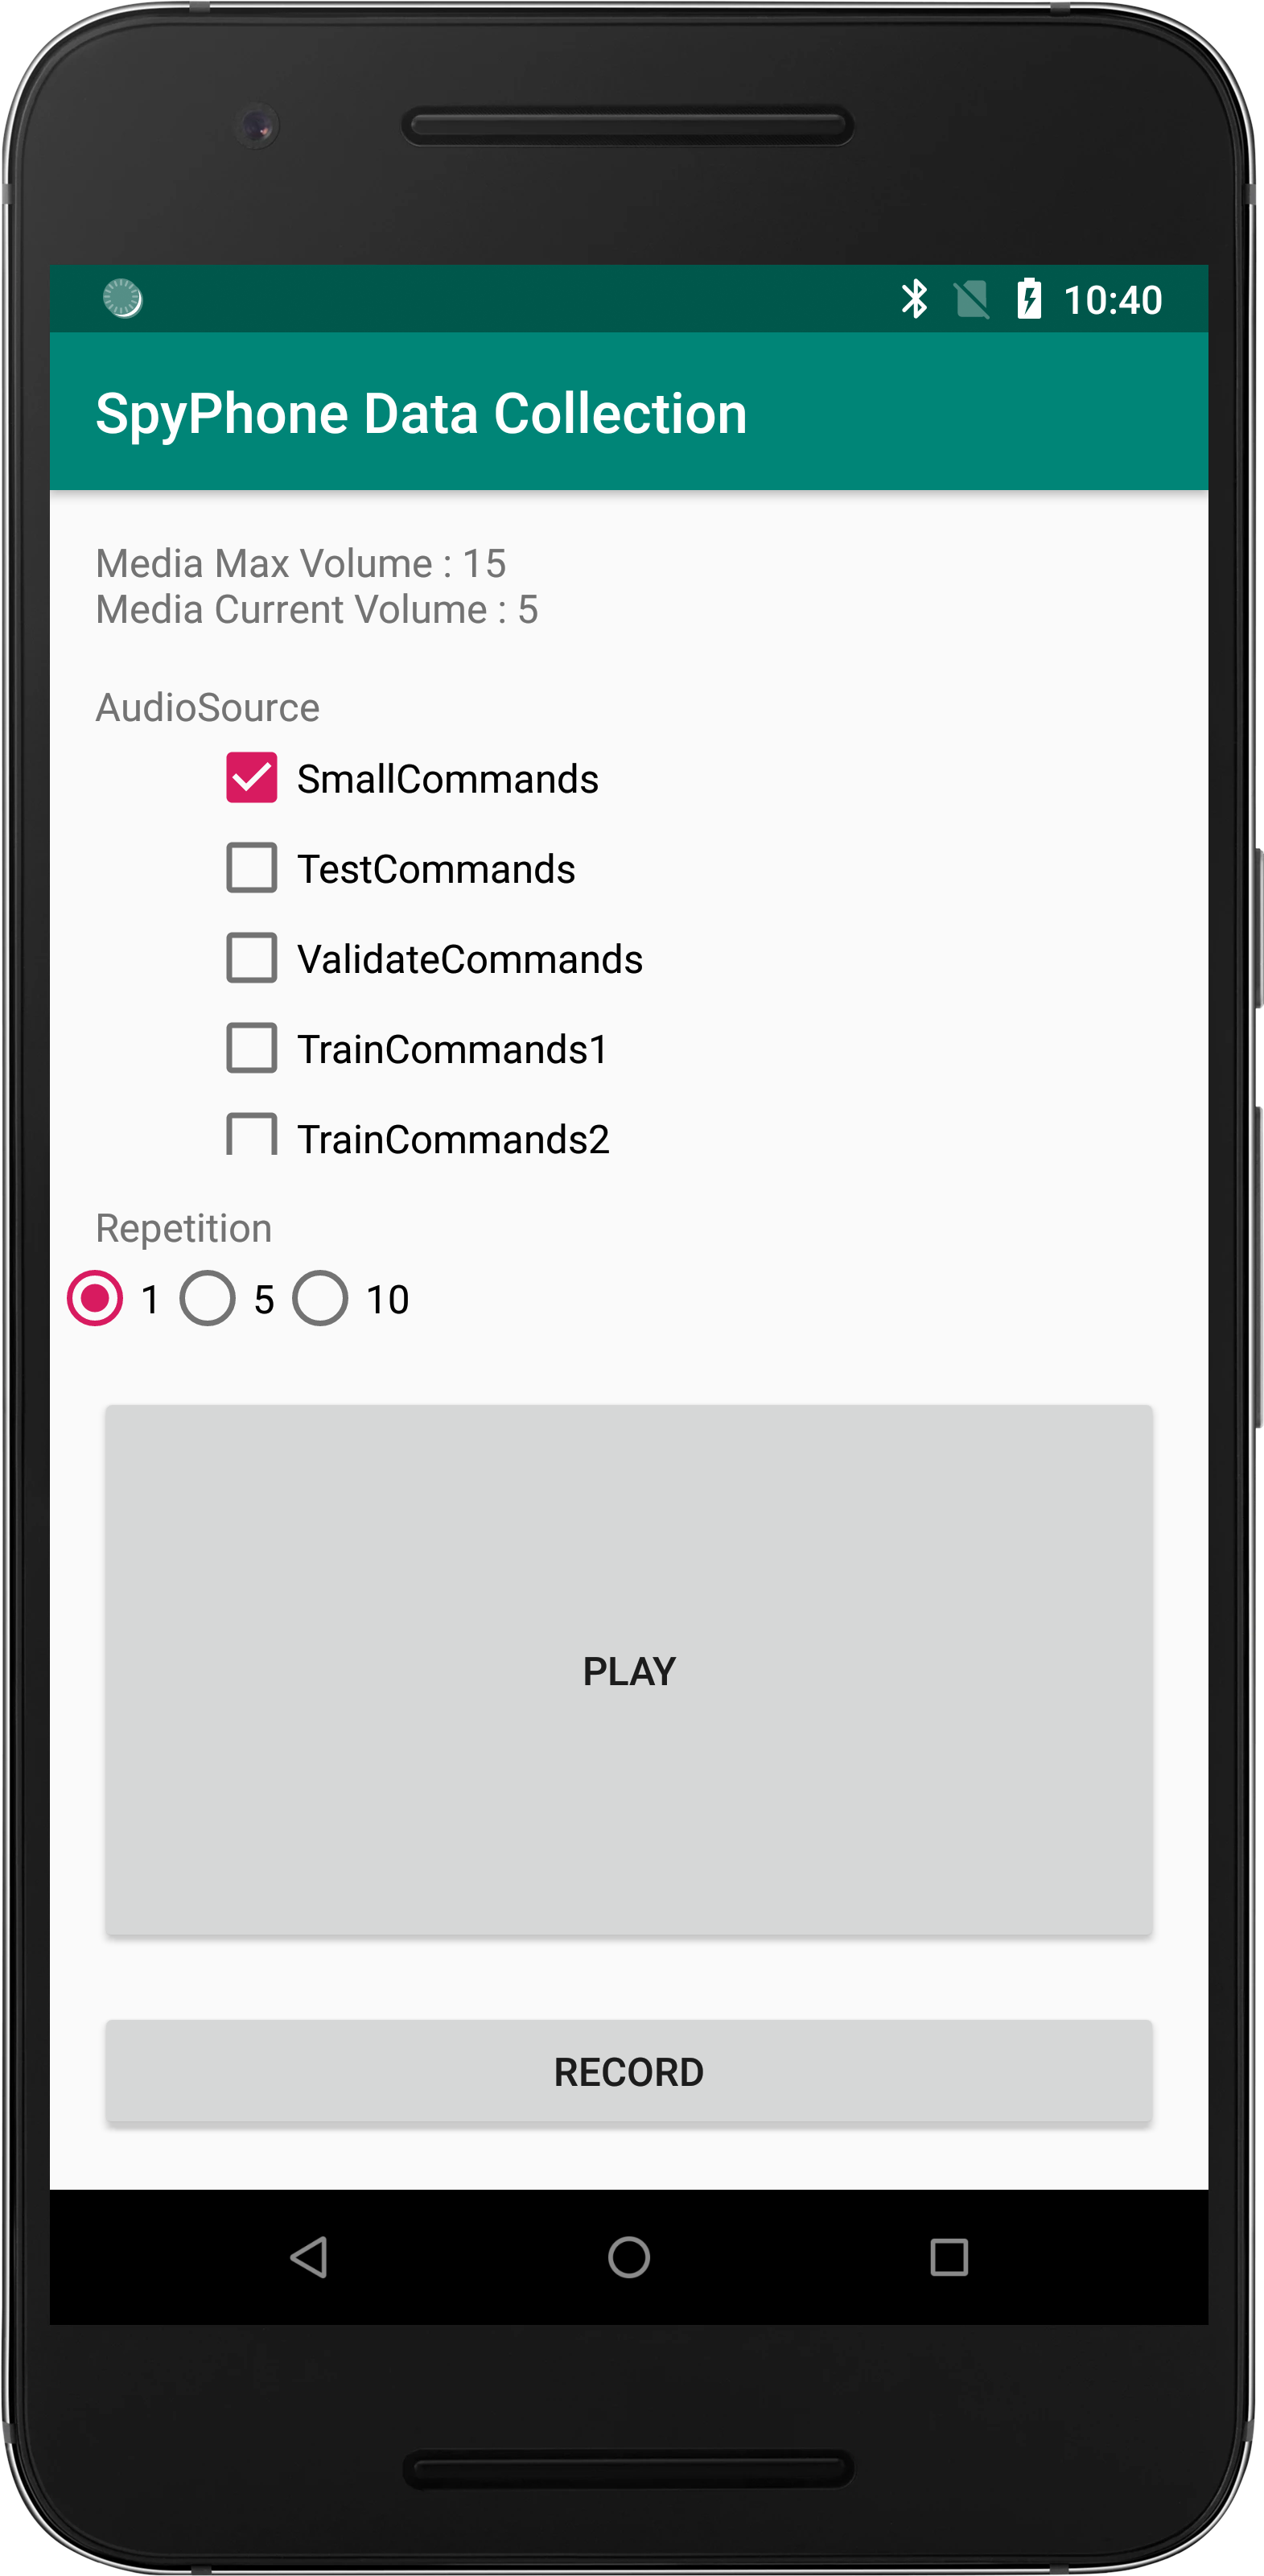
\includegraphics[height=.4\textheight]{SpyPhoneData}
	\caption{{\spp} Data Collection Application}
	\label{fig:spyphoneapp}
\end{figure}

In the beginning, the TIDIGITS dataset is used to build both the sound data and the motion data for the training dataset.
%
This corpus contains speech of 11 isolated digits: ``one'', ``two'', \ldots, ``nine'', ``zero'' and ``oh'', which are collected using an Electro-Voice RE-16 Dynamic Cardiod microphone, digitized at 20,000 Hz.
%
These audio files are directly used as training sound data. 
The motion data, however, are collected by playing these audio files using the built-in speakers of a Google Nexus 6P device. They are the simultaneous recordings from the same phone's  accelerometers and gyroscopes with a sampling rate of 400 Hz.
When playing the sound, the volume is set to be the highest level since these data will be used for training and the higher volume, the higher accuracy (according to experiments in Section~\ref{sec:impact:volume}).
Note that when the {\attackName} attack is conducted in practice, the input motion data may come from a lower volume setting defined by the user. The attacker cannot control the volume setting of the target smartphone, but she can control the volume when building the training dataset. 
%
For the training dataset, only part of the sound and motion data are used. The impact of the training data size on the prediction accuracy is elaborated in Section~\ref{sec:impact:trainsize}.
All data are collected by the SpyPhoneApp as shown in Figure~\ref{fig:spyphoneapp}.



 \begin{algorithm}[!t]
	\small
	\DontPrintSemicolon
	\LinesNumbered
	\SetKw{KwRead}{audioRead}
	\SetKw{KwRemove}{removeSilence}
	\SetKw{KwKVSD}{kvsd}
	\SetKw{KwShift}{shiftLeft}
	\SetKw{KwDown}{downSample}
	\SetKw{KwBuffer}{buffer}
	\SetKw{KwConca}{concatenate}
	\KwIn{Training Sound Dataset $\mathcal{T}_i$ for class $i$, Downsample Rate $r$, Dictionary Size $(N, K)$ }
	\KwOut{Dictionary $D_i$ for class $i$}
	$ S_i \leftarrow []$ \tcp*{Initialize training vectors} 
	\ForEach{audio file $\tau$ in $\mathcal{T}_i$}{
		\tcp{get signal $s$ and sampling frequency $fs$}
		$[s, fs] = \KwRead(\tau)$\;  
		\tcp{remove unvoiced part}
		$s\leftarrow  \KwRemove(s)$\;
		\tcp{downsample signal to $r$ subsignals and buffer each subsignal of length $N$}
		\ForEach{$j$ from 1 to $r$}{
			$s \leftarrow \KwShift(s, 1)$  \tcp*{shift left by 1 sample}  \label{line:shift}
			$ss \leftarrow \KwDown(s, r)$\; \label{line:down}
			$bs \leftarrow \KwBuffer(ss, N)$  \;
			$S_i \leftarrow \KwConca(S_i, bs)$
			
		}
		
	}
	\tcp{run K-SVD dictionary training algorithm}
	$D_i \leftarrow \KwKVSD(S_i, N, K)$
	\caption{{BuildDictionary}\label{algo:builddic}}
\end{algorithm}

\subsection{Dictionary Learning}\label{sec:design:dict}

\begin{figure*}[ht]
	\centering
	\includegraphics[width=.55\linewidth]{dict}
	\caption{Example of Learned Dictionary Atoms. For each digit class, two different atoms are shown.}\label{fig:atoms}
\end{figure*}

We now demonstrate how to construct efficient representations of audio files by building a dictionary learned from the data itself. 
Recall Section~\ref{sec:compressed}, a learned dictionary is used to reconstruct a signal when it is undersampled. 
%
In the {\systemName} system, the sound data are the signals of interest while the motion data are the measurements. The training sound data are grouped into 11 classes, (one to nine, zero, and oh). For each class $i$, the dataset is denoted by $\mathcal{T}_i$ and the representation dictionary $D_i$ is computed by Algorithm~\ref{algo:builddic}.

As shown in Figure~\ref{fig:compressed}, each representation dictionary $D_i$ is a collection of $K$ atoms, where each atom is a column vector of length $N$. An atom is basically some typical patterns of the signal of interest. For sound signal $s_i$ of class $i$,
it should be represented or approximated as a linear combination of some few of the dictionary atoms. Mathematically,
%\begin{displaymath}
	$s_i = D_i * w_i,$
%\end{displaymath} 
for each column $s_i$ in $S_i$. Here $S_i$ is the training vectors calculated in Algorithm~\ref{algo:builddic}. Compared to the original sound signal from an audio file, $S_i$ is the result from many functions including \verb|removeSilence()|, \verb|downSample()|, and \verb|buffer()|. 
 
 
 
Note that the length of a dictionary atom must be the same as the length of the training vector $s_i$. Since the original sound signal can have at most 2 s $\times$ 20,000 Hz = 40,000 samples (The duration of audio files in the dataset is at most 2 seconds.). If directly using original sound to train the dictionary, the atom size must be 40,000 as well. However, not all signals in an audio file are informative. By applying \verb|removeSilence()|, the unvoiced part of the audio signals is removed, which significantly improves the space and time efficiency of the algorithm. The \verb|removeSilence()| is based on \cite{rabiner2011theory}, which calculates the short-time energy of signals and conducts zero-crossing analysis to differentiate sounding and unvoiced parts.
 
 

Moreover, from voice acoustics elaborated in Section~\ref{sec:voice}, the most informative frequency range is roughly 100-4000~Hz, the 20,000~Hz sampling rate oversamples human speech. Therefore, to build a better representation dictionary, we shift the signals (Line~\ref{line:shift} in Algorithm~\ref{algo:builddic}) and downsample it (Line~\ref{line:down} in Algorithm~\ref{algo:builddic}) by keeping the first sample and then every $r$-th sample after the first. The impact of the downsample rate $r$ is evaluated in Section~\ref{sec:impact:downrate}.

Last but not least, different people say different digits with intrinsically different time duration, which results in different signal lengths. To build a general representation dictionary, we buffer every signal with the fixed buffer size as $N$ using \verb|buffer()|. In other words, no matter how long is the original sound signal, by Algorithm~\ref{algo:builddic}, it is transformed into a matrix $S_i$ with $N$ rows. The number of columns, however, is not fixed. For convenience's sake, we denote this number as $L_i$.




 
Dictionary Learning is the process of finding a dictionary, $D_i$ of size $N \times K$, and a corresponding coefficient matrix $W_i$ of size $K \times L_i$ such that the approximations of the training vectors, $S_i$ of size $N \times L_i$, are as good as possible, given a sparseness criterion on the coefficients. Mathematically, the dictionary learning problem can be formulated as an optimization problem with respect to $D_i$ and $W_i$:
%$
\begin{displaymath}
	\left\lbrace 
	D_{i, opt},
	W_{i, opt}
	\right\rbrace 
	=
	\argmin_{D_i, W_i}
	\sum_{l=1}^{L_i}
	\left( 
	\gamma
	\Vert w_{i, l} \Vert_p
	+
	\Vert s_{i,l} - D_i w_{i, l} \Vert_2
	\right) 
	,
%	$
\end{displaymath}
where $\gamma$ and $p$ are as in Eq.~(\ref{eq:reconstruction}), $s_{i, l}$ is the $l$-th column of $S_i$, and $w_{i, l}$ is the $l$-th column of $W_i$. 




The solver we use for this optimization problem is K-SVD~\cite{aharon2006k}, as it is one of the most well-known shared dictionary learning algorithms~\cite{xu2017survey}. We did not test all existing dictionary learning algorithms, but among those we tested, PCA~\cite{haykin2007neural}, K-SVD,  and GAD~\cite{jafari2011fast}, K-SVD provides the best results. 




K-SVD is an iterative method with two main steps: First, keep $D_i$ fixed then solve $W_i$, which is essentially $L_i$ separate problems as in Eq.~(\ref{eq:reconstruction}); Second, keep only non-zero positions in $W_i$ fixed and find $D_i$ and $W$ using singular-value decompositions (SVD). Figure~\ref{fig:atoms} shows the first two atoms in the learned dictionary of each digit class using K-SVD. Generally, the atoms are different inter-class and similar intra-class.

By concatenating every $D_i$ together, the overall dictionary is 
\begin{equation}
	D = \left[ D_1, D_2, \ldots, D_i, \ldots, D_{11} \right], \label{eq:dictConcat}
\end{equation}
which will be used for signal reconstruction in later steps.





\subsection{Motion Data Preprocessing}
The input motion data are collected similarly to how motion data are collected for the training dataset, i.e., playing TIDIGITS audio files by the smartphone's built-in speakers. However, since these data are to simulate the attacking scenarios in reality, the data are collected multiple times using 15 different volume settings (Section~\ref{sec:impact:volume}). Moreover, we collected the motion data in both quiet and noisy environment (Section~\ref{sec:impact:noise}), and in both stable and moving states (Section~\ref{sec:impact:move}).
\begin{figure*}[!h]
	\centering
	\includegraphics[width=.8\linewidth]{preprocess0}
	\caption{The Magnitude and Phase Response of the FIR Highpass filter.}\label{fig:spyphoneresponse}
\end{figure*}


\begin{figure}[H]
	\begin{minipage}[t]{.45\linewidth}
		\centering
		\includegraphics[width=\linewidth]{preprocess1}
		\includegraphics[width=\linewidth]{preprocess2}
		\vspace{-.2in}
		\subcaption{Raw Motion Data.}\label{fig:rawmotion}
		\vspace{.2in}
		\includegraphics[width=\linewidth]{preprocess3}
		\vspace{-.2in}
		\subcaption{Spectrogram of Raw Motion Signals.}\label{fig:rawspec}
	\end{minipage}
	\begin{minipage}[t]{.05\linewidth}
		\quad
	\end{minipage}
	%\end{figure}
	%
	%\begin{figure}\ContinuedFloat	
	\begin{minipage}[t]{.45\linewidth}
		\centering
		\includegraphics[width=\linewidth]{preprocess4}
		\vspace{-.2in}
		\subcaption{Spectrogram of Proceseed Signals.}\label{fig:newspec}
		\vspace{.2in}
		\includegraphics[width=\linewidth]{preprocess5}
		\includegraphics[width=\linewidth]{preprocess6}
		\vspace{-.2in}
		\subcaption{Preprocessed Motion Data}\label{fig:newmotion}
	\end{minipage}
	
	\caption[Preprocessing of Motion Data. ]{Preprocessing of Motion Data. The top two figures show the raw data from 3-axis accelerometers and 3-axis gyroscopes. There are 450 samples shown in the figure. These samples span about one second (450 / 400Hz = 1.125s) and are collected when the user is dropping the head of the phone while playing a ``Zero'' utterance from a male speaker. The frequency of such movement is far less than the frequency of human voices. Therefore, by applying the high pass filter, the noise caused by hand movements will be removed. }
	
	\label{fig:spyphonepreprocess}
\end{figure}

As mentioned in Section~\ref{sec:intro}, the motion data is impeded by low sampling rates, weak target signals, and large  interference  noises. To overcome such problems, we must preprocess the motion data. We apply a high pass filter to mitigate the noise and increase the signal-to-noise ratio. The cutoff frequency is set to be 50 Hz, since noises such as walking or other human body movements are unlikely to generate signals as high as 50 Hz.
We also use the speech-background separation algorithms from \cite{rabiner2011theory} to differentiate the data affected by sound signals from those do not. The red vertical lines in Figure~\ref{fig:rawmotion} are the borderlines between the speech part and the background part. 
Figure~\ref{fig:rawspec} and Figure~\ref{fig:newspec} show that various noises can be removed by applying a high pass filter.
The result after the preprocessing stage is shown in Figure~\ref{fig:newmotion}. These data will be used in the next signal reconstruction stage.



\subsection{Signal Reconstruction}
In this stage, the preprocessed motion data will be used to reconstruct the original audio data.

Mathematically, the goal of signal reconstruction is to solve $w^\prime$ in 
%$$$$ 
%\vspace{-.2in}
%\begin{displaymath}
	$x = R \times w^\prime$
%\end{displaymath}
as in Figure~\ref{fig:compressed}. Here the measurement $x$ is the motion data after preprocessing, and the reconstruction matrix $R$ is calculated by
\begin{equation}
R = S \times D, \label{eq:reconstruct2}
\end{equation}
where $S$ is the sensing matrix and $D$ is the dictionary obtained in Section~\ref{sec:design:dict}.

In the {\systemName} system, the sensing matrix describes the sensing procedure from audio data to motion data, which can be regarded as a downsampling operation. The downsampling rate ($r$) is determined by the sampling frequencies of smartphone speakers ($f_1$) and motion sensors ($f_2$): $r = f_1/f_2$. For example, a sensing matrix with downsample rate $r=3$ is as follows:
\begin{displaymath}
\small
S = 
\begin{bmatrix} 
1 & 0 & 0 & 0 & 0 & 0 & 0 & \cdots & 0  & 0& 0\\
0 & 0 & 0 & 1 & 0 & 0 & 0 & \cdots & 0 & 0& 0\\
0 & 0 & 0 & 0 & 0 & 0 & 1 & \cdots & 0 & 0& 0\\
\vdots & \vdots & \vdots & \vdots & \vdots & \vdots & \vdots &  & \vdots & \vdots & \vdots\\
0 & 0 & 0 & 0 & 0 & 0 & 0 & \cdots & 1 & 0& 0\\       
\end{bmatrix}.
\end{displaymath}
%
In the {\systemName} system, the true value of this rate can be as high as 48,000~/~ 400~ = 120, which indicates a huge information loss and a big challenge to recover the signals.
%
Note that Algorithm~\ref{algo:builddic} also has a downsampling operation (Line~\ref{line:down}), therefore the $R=S \times D$ operation can be replaced by changing the parameter $r$ in Algorithm~\ref{algo:builddic}. When reconstructing the signals, $D$ is used as $R$. The impact of the downsample rate $r$ is evaluated in Section~\ref{sec:impact:downrate}.
%
To solve Eq.~(\ref{eq:reconstruct2}), GPSR~\cite{figueiredo2007gradient} is used, which is able to find  
$
%\begin{displaymath}
w^\prime_{opt}
=
\argmin_{w^\prime}
\left( 
\gamma
\Vert w^\prime \Vert_p
+
\Vert x - R w^\prime \Vert_2
\right)
. 
$
%\end{displaymath}
The last step is to reconstruct the signal of interests by
$
%\begin{displaymath}
s^\prime = D \times w^\prime_{opt}.
%\end{displaymath}
$
These signals will be used as training data for the Bi-LSTM network discussed in the next section.




\begin{figure}[!b]
	\centering
	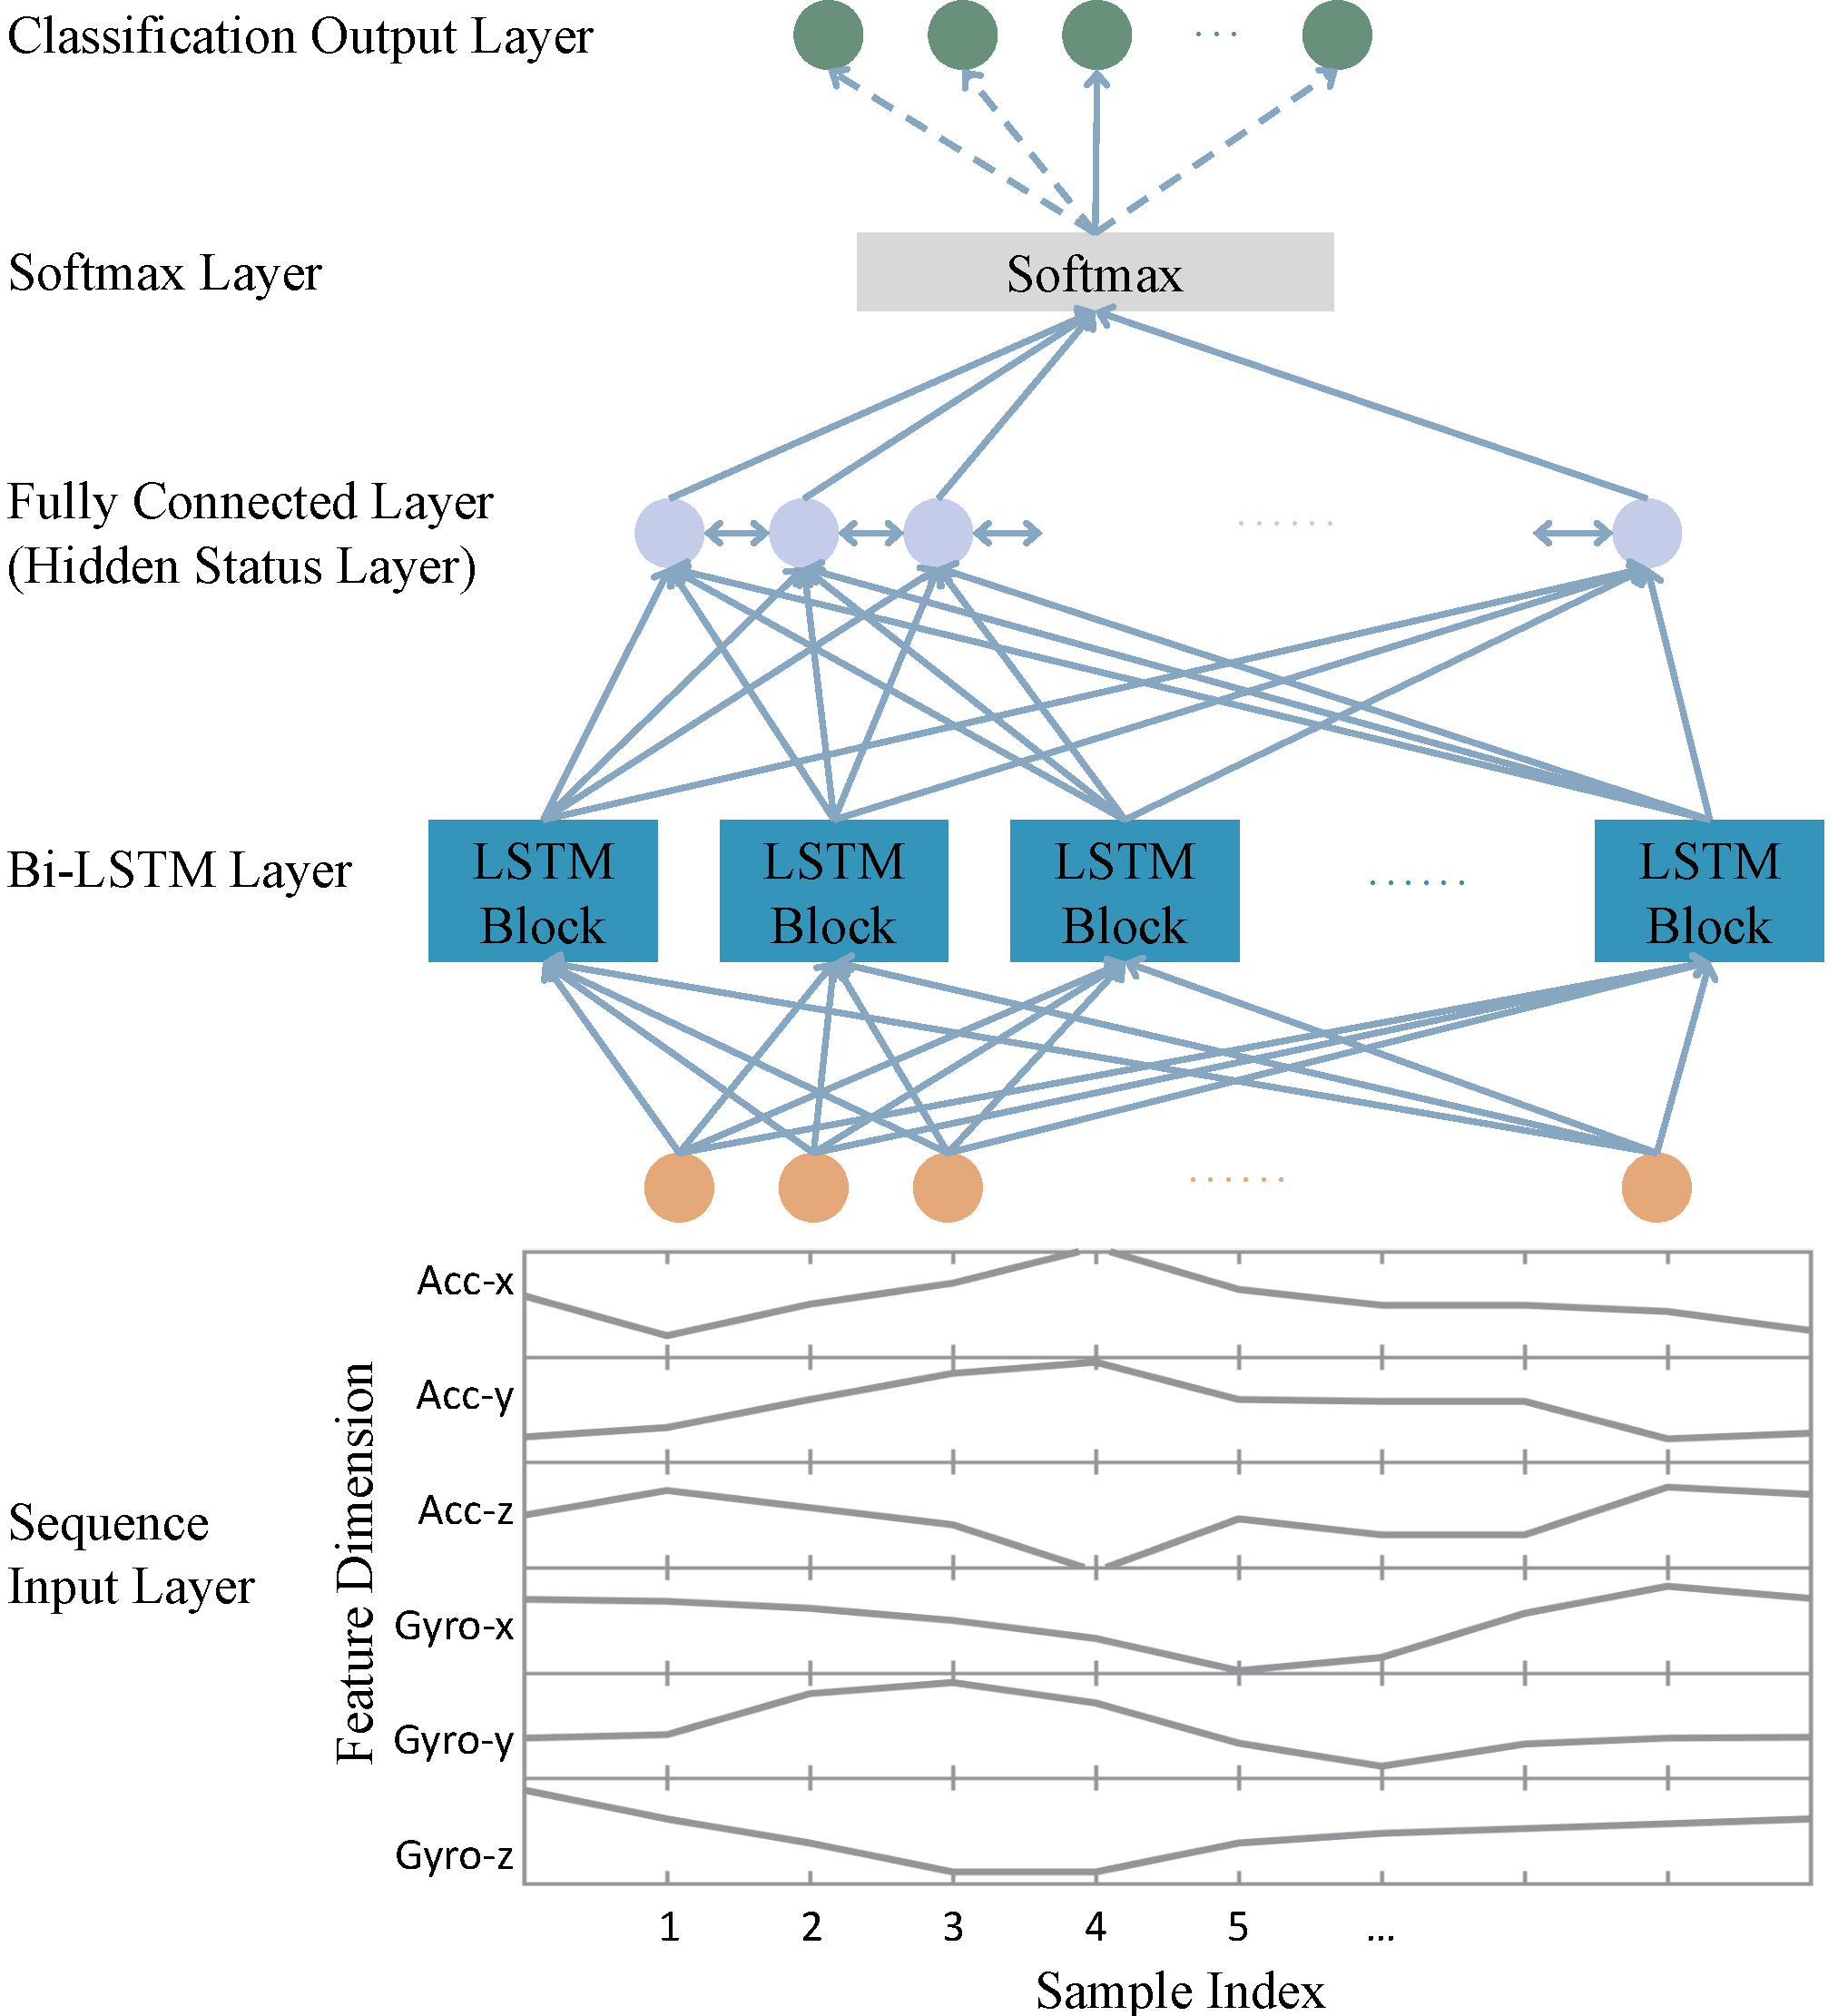
\includegraphics[width=.65\linewidth]{rnn}
	\caption{The Bidirectional Long Short-Term Memory Network (Bi-LSTM Network).}
	\label{fig:rnn}
\end{figure}


\subsection{Bi-LSTM Learing}\label{sec:LSTM}

The last stage is to use the reconstructed data to establish a Bi-directional Long Short-Term Memory (Bi-LSTM) network model, which will be used for classifying the input data later on.
%
 LSTM was first proposed by Sepp Hochreiter and J{\"u}rgen Schmidhuber in 1997 ~\cite{hochreiter1997long}. It is a special variant of  Recurrent Neural Networks (RNN), and is widely used in learning, processing, and classifying \textit{sequential } data because of 
its great property of selectively remembering patterns for long durations of time. 
%
Over the years, there have also been many variants of LSTM networks. However, based on a study in 2017, none of the variants can improve upon the standard LSTM architecture significantly~\cite{greff2017lstm}. Therefore, we still choose to implement the standard LSTM network in this work except for the bi-directional calculation. The original unidirectional LSTM network only preserves information from the inputs seen in the past. Bi-LSTM network, on the contrary, preserves information both from the past and the future. 
%
As shown in Figure~\ref{fig:rnn}, our Bi-LSTM network has five layers in total. In the sequence input layer, the input data have 6 feature dimensions, which consists of 3 accelerometer dimensions and 3 gyroscope dimensions. Then we establish an LSTM layer formed by LSTM blocks, where each block publishes its cell state to the next LSTM block. The output of the LSTM layer is sent to the fully connected hidden status layer. We set the total number of hidden units to be 100, and each hidden unit has two hidden states, one from the past and the other from the future. Then we feed the combined hidden status to a softmax function and output the classification results.





	
%

\section{Feasibility Experiments }\label{sec:experiment}

In this section, we validate the {\systemName} system and show it can eavesdrop on smartphone's built-in speakers and obtain critical information discussed in Section~\ref{sec:threat}. 


\begin{landscape}
	\centering
	\begin{table}[h]
		\caption{Comparison with Prior Works}
		\label{tab:comparison}
		\centering
		%		\resizebox{\textwidth}{!}{
		\begin{tabular}{cccccc}
			\toprule[1pt]\midrule[0.3pt]
			Work & Sensors & Setting & Main Techniques & Classification Classes & Accuracy\\
			\midrule[0.5pt]
			\multirow{4}{*}{\shortstack{~~~Gyrophone \\ ~~\cite{michalevsky2014gyrophone}}}& \multirow{4}{*}{Gyroscopes} & \multirow{4}{*}{\parbox{3cm}{\centering 10 people from TIDIGITS \\ Desktop\\ Loudspeakers}} & \multirow{4}{*}{\parbox{1.8cm}{\centering SVM\\ GMM\\ DTW}} & \multirow{2}{*}{1 to 9, Oh, Zero (11)}& Speaker-independent: 26\% \\ 
			&&&&& Speaker-dependent: 65\%\\ \cline{5-6}
			&&&&Speaker Identification& 65\%\\ \cline{5-6}
			&&&&Speaker Gender& 84\%\\
			\midrule[0.5pt]
			\multirow{3}{*}{\shortstack{~Accelword \\ ~~\cite{zhang2015accelword}}} & \multirow{3}{*}{Accelerometers }&\multirow{3}{*}{10 people} & \multirow{3}{*}{\parbox{1.8cm}{\centering Decision Tree} } & \multirow{2}{*}{\parbox{4cm}{\centering Ok Google, Hi Galaxy, Others (3)}}&\multirow{2}{*}{Speaker-dependent: 85\%}\\
			&&&&&\\ \cline{5-6}
			&&&&Speaker Identification & 86\%\\
			\midrule[0.5pt]
			\multirow{4}{*}{\shortstack{~~SpearPhone \\ ~~\cite{anand2019spearphone}}}& \multirow{4}{*}{Accelerometers} & \multirow{4}{*}{\parbox{3.5cm}{\centering 326 people from TIDIGITS \\Built-in Speakers \\in Smartphones}} & \multirow{4}{*}{\parbox{3cm}{\centering SVM with SMO\\ Logistic\\RF \\ RT}} & \multirow{2}{*}{1 to 9, Oh, Zero (11)}& \multirow{2}{*}{Speaker-dependent: 71\%} \\ 
			&&&&& \\ \cline{5-6}
			&&&&Speaker Identification& 80\%\\ \cline{5-6}
			&&&&Speaker Gender& 90\%\\
			\midrule[0.5pt]
			\multirow{4}{*}{~~~\systemName} & \multirow{4}{*}{Both} & \multirow{4}{*}{\parbox{3.5cm}{\centering 326 people from TIDIGITS \\Built-in Speakers \\in Smartphones}} & \multirow{4}{*}{\parbox{1.8cm}{\centering Compressed Sensing\\Bi-LSTM} } &1 to 9, Oh, Zero (11) &Speaker-independent: 90\%\\ \cline{5-6}
			&&&&User Activity& 81\%\\ \cline{5-6}
			&&&&Speaker Identification& 98\%\\ \cline{5-6}
			&&&&Speaker Gender& 93\%\\
			\midrule[0.3pt]\bottomrule[1pt]
		\end{tabular}
		%	}
	\end{table}
\end{landscape}

%
The main result and the comparison to prior works are summarized in Table~\ref{tab:comparison}. 


\subsection{Speech Content Learning  (Digits)}

The TIDIGITS dataset~\cite{leonard1993tidigits} has 7172 audio files of isolated digits. We use 3586 of them (3586~/~7172 =50\%) to train the dictionary. With the downsample rate $r$ set to 40, dictionary size set to ($N$=400, $K$=10), and the $p$-norm set to be the $\ell_1$-norm (absolute value), we learn an overall dictionary of size 400~$\times$~110 by concatenating each dictionary of each individual digit class. 
%
For each audio file, we play it by smartphones' built-in speakers for 30 times. Therefore, the size of the motion data is actually 30 times of the size of the sound data in the training dataset. The Bi-LSTM network is actually trained with 3586~$\times$~30=107,580 data, which are the resulted signals after preprocessing and signal reconstruction. Note that although this number seems big, each data is just 1-second data at a sampling rate of 400 Hz, and each sample is 16 bits. So the total size is 107,580~$\times$~400~$\times$~16 = 688,512,000 bits = 86.1 MB, which is indeed not big at all.


%%%TODO
%result or results
\begin{figure}[!h]
	\centering
	\includegraphics[width=.8\linewidth]{digitCFM}
	\centering
%	\resizebox{\linewidth}{!}{
		\begin{tabular}{lr}
		\toprule
		Accuracy: 90.13\% & \hspace{-.55in} Error Rate: 9.87\% \\
		Precision: 90.13\% & \hspace{-.55in} True Positive Rate (Sensitivity/Recall): 90.71\% \\
		$F_1$ Score: 0.901 & \hspace{-.55in} True Negative Rate (Specificity): 99.02\% \\
		False Negative Rate: 9.29\% & \hspace{-.55in} False Positive Rate: 0.98\% \\
		\bottomrule
	\end{tabular}

	\caption{The Confusion Matrix of the Digit Classification Result.}
	\label{fig:digitCFM}
\end{figure}
%\vspace{-.1in}
%confusion matrix
%
The test data is motion data from the remaining 3586 audio files. This data has never been seen by the Bi-LSTM network before. The classification result is shown as a confusion matrix in Figure~\ref{fig:digitCFM}. In the confusion matrix, each row of the matrix represents the instances in a predicted/output class while each column represents the instances in an actual/target class. The digit class ``zero'' has the highest classification accuracy of 98.6\%. The digit class ``eight'' has the lowest accuracy: only 70.5\% instances are classified to the correct class, while 16.2\% are classified as ``six''.
The overall accuracy of all 11 classes is 90.13\%, with a sensitivity (true positive rate) of 90.13\% and a specificity (true negative rate) of 99.02\%.


\subsection{Speech Content Learning (Commands)}\label{sec:word}
The TensorFlow Speech Commands Dataset Version 2~\cite{warden2018speech} was used for limited-vocabulary speech recognition. This dataset consists of 105,829 utterances of 35 words such as forward, house, happy, etc. A random guessing provides accuracy of 1/35 = 2.9\%, but {\systemName} could achieve 73.4\%. The accuracy is relatively lower than TIDIGITS, as TIDIGITS are professionally recorded while the commands data are crowdsourced online. Using the original 16,000 Hz audio data can only achieve accuracy of 88.2\%~\cite{warden2018speech}. {\systemName} (using 400 Hz motion data) has the correct rate of 73.4/88.2=83.2\%.

\subsection{Speaker Gender Classification and Speaker Identification}


\begin{figure}[!h]
	\begin{minipage}{\linewidth}
			\centering
		\begin{minipage}[c]{0.35\linewidth}
			
			\includegraphics[width=.9\linewidth]{digitCFMGender}
		\end{minipage}
%	\hfill
		\begin{minipage}[b]{0.49\linewidth}
			 \centering
				\begin{tabular}{r}
				\toprule
				Accuracy: 93.15\% \\ Error Rate: 6.85\% \\
				Precision: 99.19\% \\True Positive Rate : 88.28\% \\
				$F_1$ Score: 0.934 \\ True Negative Rate: 99.12\% \\
				False Negative Rate: 11.72\% \\ False Positive Rate: 0.88\% \\
				\bottomrule
			\end{tabular}
%		}
		\end{minipage}
	\end{minipage}
\caption{The Confusion Matrix of the Speaker Gender Classification Result. 
		}
%		The total number of instances of true class ``Female'' is 114$\times$11$\times$2=2508, while that of ``Male'' is 93$\times$11$\times$2=2046.}
	\label{fig:genderCFM}
\end{figure}

\begin{table}[!h]
	\caption{Statistical Analysis of the Speaker Identification Result.}
	\label{tab:idTable}
	\centering	
%	\small 
	\centering
%		\vspace{-.1in}
%	\resizebox{\linewidth}{!}{
		\begin{tabular}{lr}
		\toprule
		Accuracy: 97.56\% & \hspace{-.2in} Error Rate: 2.44\% \\
		Precision: 97.69\% & \hspace{-.2in} True Positive Rate (Sensitivity/Recall): 97.56\% \\
		$F_1$ Score: 0.976 & \hspace{-.2in} True Negative Rate (Specificity): 99.99\% \\
		False Negative Rate: 2.44\% & \hspace{-.2in} False Positive Rate: 0.01\% \\
		\bottomrule
	\end{tabular}
%}
%	\vspace{-.1in}
\end{table}

The same training and testing data are also used for gender classification and speaker identification, since the TIDIGITS audio files are labeled with gender and speaker ID. The result for gender classification is shown in Figure~\ref{fig:genderCFM}.
For speaker identification, since the number of classes is 225, we do not show the confusion matrix, but show the result of statistical analysis as in Table~\ref{tab:idTable}. The overall accuracy is 97.56\% with the sensitivity of 97.56\% and the specificity is 99.99\%.




\subsection{User Activity Classification (Sound Type)}


We also test whether the {\systemName} can classify the type of sound signals played by smartphone speakers. The dataset consists of two parts: the first is the built-in (default) alarm sounds, notification sounds and ringtones provided by the Android operating system, the other is the speech sounds from the TIMIT~\cite{garofolo1993timit} dataset where 10 sentences are spoken by each speaker.
%
In detail, we obtain 18 alarm sounds, 11 notification sounds, and 12 ringtones from \verb|/system/media/sound/| on a Google Nexus 6P smartphone with an Android 8.1 ``Oreo'' system. The speech data consist of 10 sentences from a male speaker and 10 sentences from a female speaker. We increase the atom size $N$ to 800 when building the dictionary, so that the measurement size is 800 as well, which means a piece of motion data of 800~/~400 Hz = 2~seconds. In other words, when classifying the sound type, we evaluate the motion data using a 2-second threshold, which is longer than that of classifying the digit (1~second).


\begin{figure}[ht]
	\begin{minipage}{\linewidth}
		\centering
		\begin{minipage}[c]{0.5\linewidth}			
			\includegraphics[width=.8\linewidth]{activityCFM}
		\end{minipage}
		%	\hfill
		\begin{minipage}[b]{0.49\linewidth}
			\centering
			%			\resizebox{\linewidth}{!}{
			\begin{tabular}{r}
				\toprule
				Accuracy: 80.56\% \\ Error Rate: 19.44\% \\
				Precision: 72.22\% \\ True Positive Rate: 72.49\% \\
				$F_1$ Score: 0.720\\ True Negative Rate: 94.07\% \\
				False Negative Rate: 27.51\% \\ False Positive Rate: 5.93\% \\
				\bottomrule
			\end{tabular}
			%		}
		\end{minipage}
	\end{minipage}
	
	\vspace{-.1in}
	\caption{The Confusion Matrix of the Sound Type Classification Result.}
	\label{fig:activityCFM}
	\vspace{-.1in}
\end{figure}

The result is shown in Figure~\ref{fig:activityCFM}.
 The {\systemName} system can successfully differentiate between different sound types with an overall accuracy of 80.56\%, which means attackers can know when you get up in the morning (``Alarm''), when you receive a notification (``Notification''), when you are called by others (``Ringtone''), and when the person from the other end of call starts speaking (``Ringtone'' followed by ``Speech''). Moreover, attackers can also infer activities such as watching videos or listening to audio-books (``Speech'' without ``Ringtone'' as a precursor). In other words, various sound-related user activities are not secrets to {\attackName} attackers, not to mention that motion-related activities can be monitored by motion sensors as a default.
%
Note that the average accuracy of identifying ``speech'' is 94.7\%, so the {\systemName} system can first determine whether the input belongs to ``speech'', then classify the speaker gender/identity or the digit class as mentioned above. 


The overall accuracy is much lower because of the other three classes. These classes are misclassified since alarm sounds, notification sounds and ringtones are not strictly defined. Android groups them in a generally conventional way, not by scientific methods. In fact, smartphone users may choose to use ringtones as alarms, or use alarm sounds as ringtones. Such inherent ambiguity is the main reason for the low accuracy. To further improve the accuracy, more features such as the total duration (``notification'' tends to be shorter than ``ringtones'') or the repetitive (``alarm'' tends to ring once a day) should be considered. Integrating algorithms to learn these features is a potential future work for a better design of {\systemName}.


	
%
\section{Impact Evaluation}\label{sec:impact}
In this section, we evaluate the impact of two internal parameters and three external parameters on the performance of the {\systemName} system for digit classification. 
The internal parameters control how the dictionary is learned and the external parameters control the quality of input motion data. 
%All the following experiments perform digit classification. Therefore, 
Note that a random guess results in an accuracy of 1/11 = 9.09\%.

\subsection{Impact of Training Data Size}\label{sec:impact:trainsize}
\begin{figure}[h]
	\centering
	\includegraphics[width=.5\linewidth]{trainSize}
	\vspace{-.1in}
	\caption{Impact of Training Data Size.}
	\label{fig:trainSize}
	\vspace{-.1in}
\end{figure}

The size of training data for dictionary learning is an internal parameter. In the previous section, we use 3586 audio files (50\% of full dataset) to train the dictionary. In this section, we vary the size from 660 to 1760 and show the experiment results in Figure~\ref{fig:trainSize}, which is a box and whisker plot\footnote{The ends of the box are the upper and lower quartiles (25th and 75th percentiles), the central line inside the box indicates the median, the whiskers extend to the highest and lowest accuracy values not considered outliers, and the outliers are plotted individually using the `+' symbol.}. 
We can see that the classification accuracy increases from $\sim$56\% to $\sim$78\% as the data size increases. This result is reasonable since the more data is used in training, the learned dictionary is more representative and the machine learning model is more accurate. 
%
In fact, recent researches have shown that to build a representation dictionary, the typically sufficient number of training samples grows up quasilinearly with the signal dimension, i.e., $\mathcal{O}(N\log N)$~\cite{remi2010dictionary}. In our experiment, the atom size $N$ is set to be 400, therefore, several hundred or a few thousand of training data should be enough.




\subsection{Impact of Downsampling Rate}\label{sec:impact:downrate}
\begin{figure}[h]
	\centering
	\includegraphics[width=.6\linewidth]{downsample}
	\vspace{-.1in}
	\caption{Impact of Downsampling Rate.}
	\label{fig:downsampling}
	\vspace{-.1in}
\end{figure}

The downsampling rate $r$ is the other internal parameter to study. This parameter is influenced by four frequencies: the sampling rate of smartphones' built-in speakers (48,000~Hz in Nexus 6P), the sampling rate to record human speech (20,000 Hz in TIDIGIT), the frequency range of human speech (100-4,000~Hz), and the sampling rate of motion sensors (400 Hz in Nexus 6P). 
%
We vary this rate from 5 to 50 and find that the performance of {\systemName} improves with the increase of the downsampling rate at the beginning, then the accuracy enters a relatively stable stage when $r=30$ and $r=40$. The accuracy declines if a higher downsampling rate is used ($r=50$). From Figure~\ref{fig:downsampling}, when $r \in [20, 50]$, the average accuracy is above 90\%. 
%
We do not test the cases when $r > 50$, because $50 = 20,000 Hz / 400 Hz$ is the gap between the sampling rate of training sound data and that of motion data. If we use a larger downsampling rate, the learned atoms would contain less information than the motion data, which invalidates the dictionary and contradicts with the goal of using compressed sensing to reconstruct more signal samples. 




\subsection{Impact of Training Device}\label{sec:impact:device}
We tested whether the trained LSTM network is robust across different devices. Due to time limit, only two devices are tested with the result shown in Table~\ref{tab:device}. Different devices with same model, and different devies with different model will be tested as a future work.
\begin{table}[!h]
	\caption{Statistical Analysis of the Speaker Identification Result.}
	\label{tab:device}
	\centering	
%	\small 
	\centering
%	\vspace{-.1in}
	\begin{tabular}{ccc}
		\toprule[0.5pt]
		& Nexus 6P Training& Galaxy S8 Training\\
		\midrule[0.5pt]
		Nexus 6P Testing & 90.52\% & 83.26\%\\
		Galaxy S8 Testing & 84.39\% & 90.48\% \\
		\bottomrule[0.5pt]
	\end{tabular}
%	\vspace{-.1in}
\end{table}

\subsection{Impact of Sound Volume}\label{sec:impact:volume}
\begin{figure}[!h]
	\centering
	\includegraphics[width=.9\linewidth]{volume}
	\caption{Impact of Sound Volume.}
	\label{fig:volume}
\end{figure}


In this section, we study how the sound volume affects the performance of {\systemName}. 
%
By calling the \verb|getStreamVolume(AudioManager.STREAM_MUSIC)| for the \verb|AudioManager| class, the Google Nexus 6P device supports 15 volume levels. All these volume levels are tested and the results are shown in Figure~\ref{fig:volume}. 
%
The accuracy goes up when the volume goes up. The classification accuracy is above 60\% when the volume is set to be level 10 or larger, and the accuracy goes to above 90\% when the volume is set to be the highest two levels. Even when the volume is low, the average accuracy is about 30-40\%, over 3 times higher than the random guess accuracy of 9.09\%.


\subsection{Impact of Surrounding Environment}\label{sec:impact:noise}

\begin{figure}[ht]
	\centering
	\includegraphics[width=.6\linewidth]{noise}
	\caption{Impact of Surrounding Environment.}
	\label{fig:noise}
\end{figure}

\begin{figure}[!h]
	\centering
	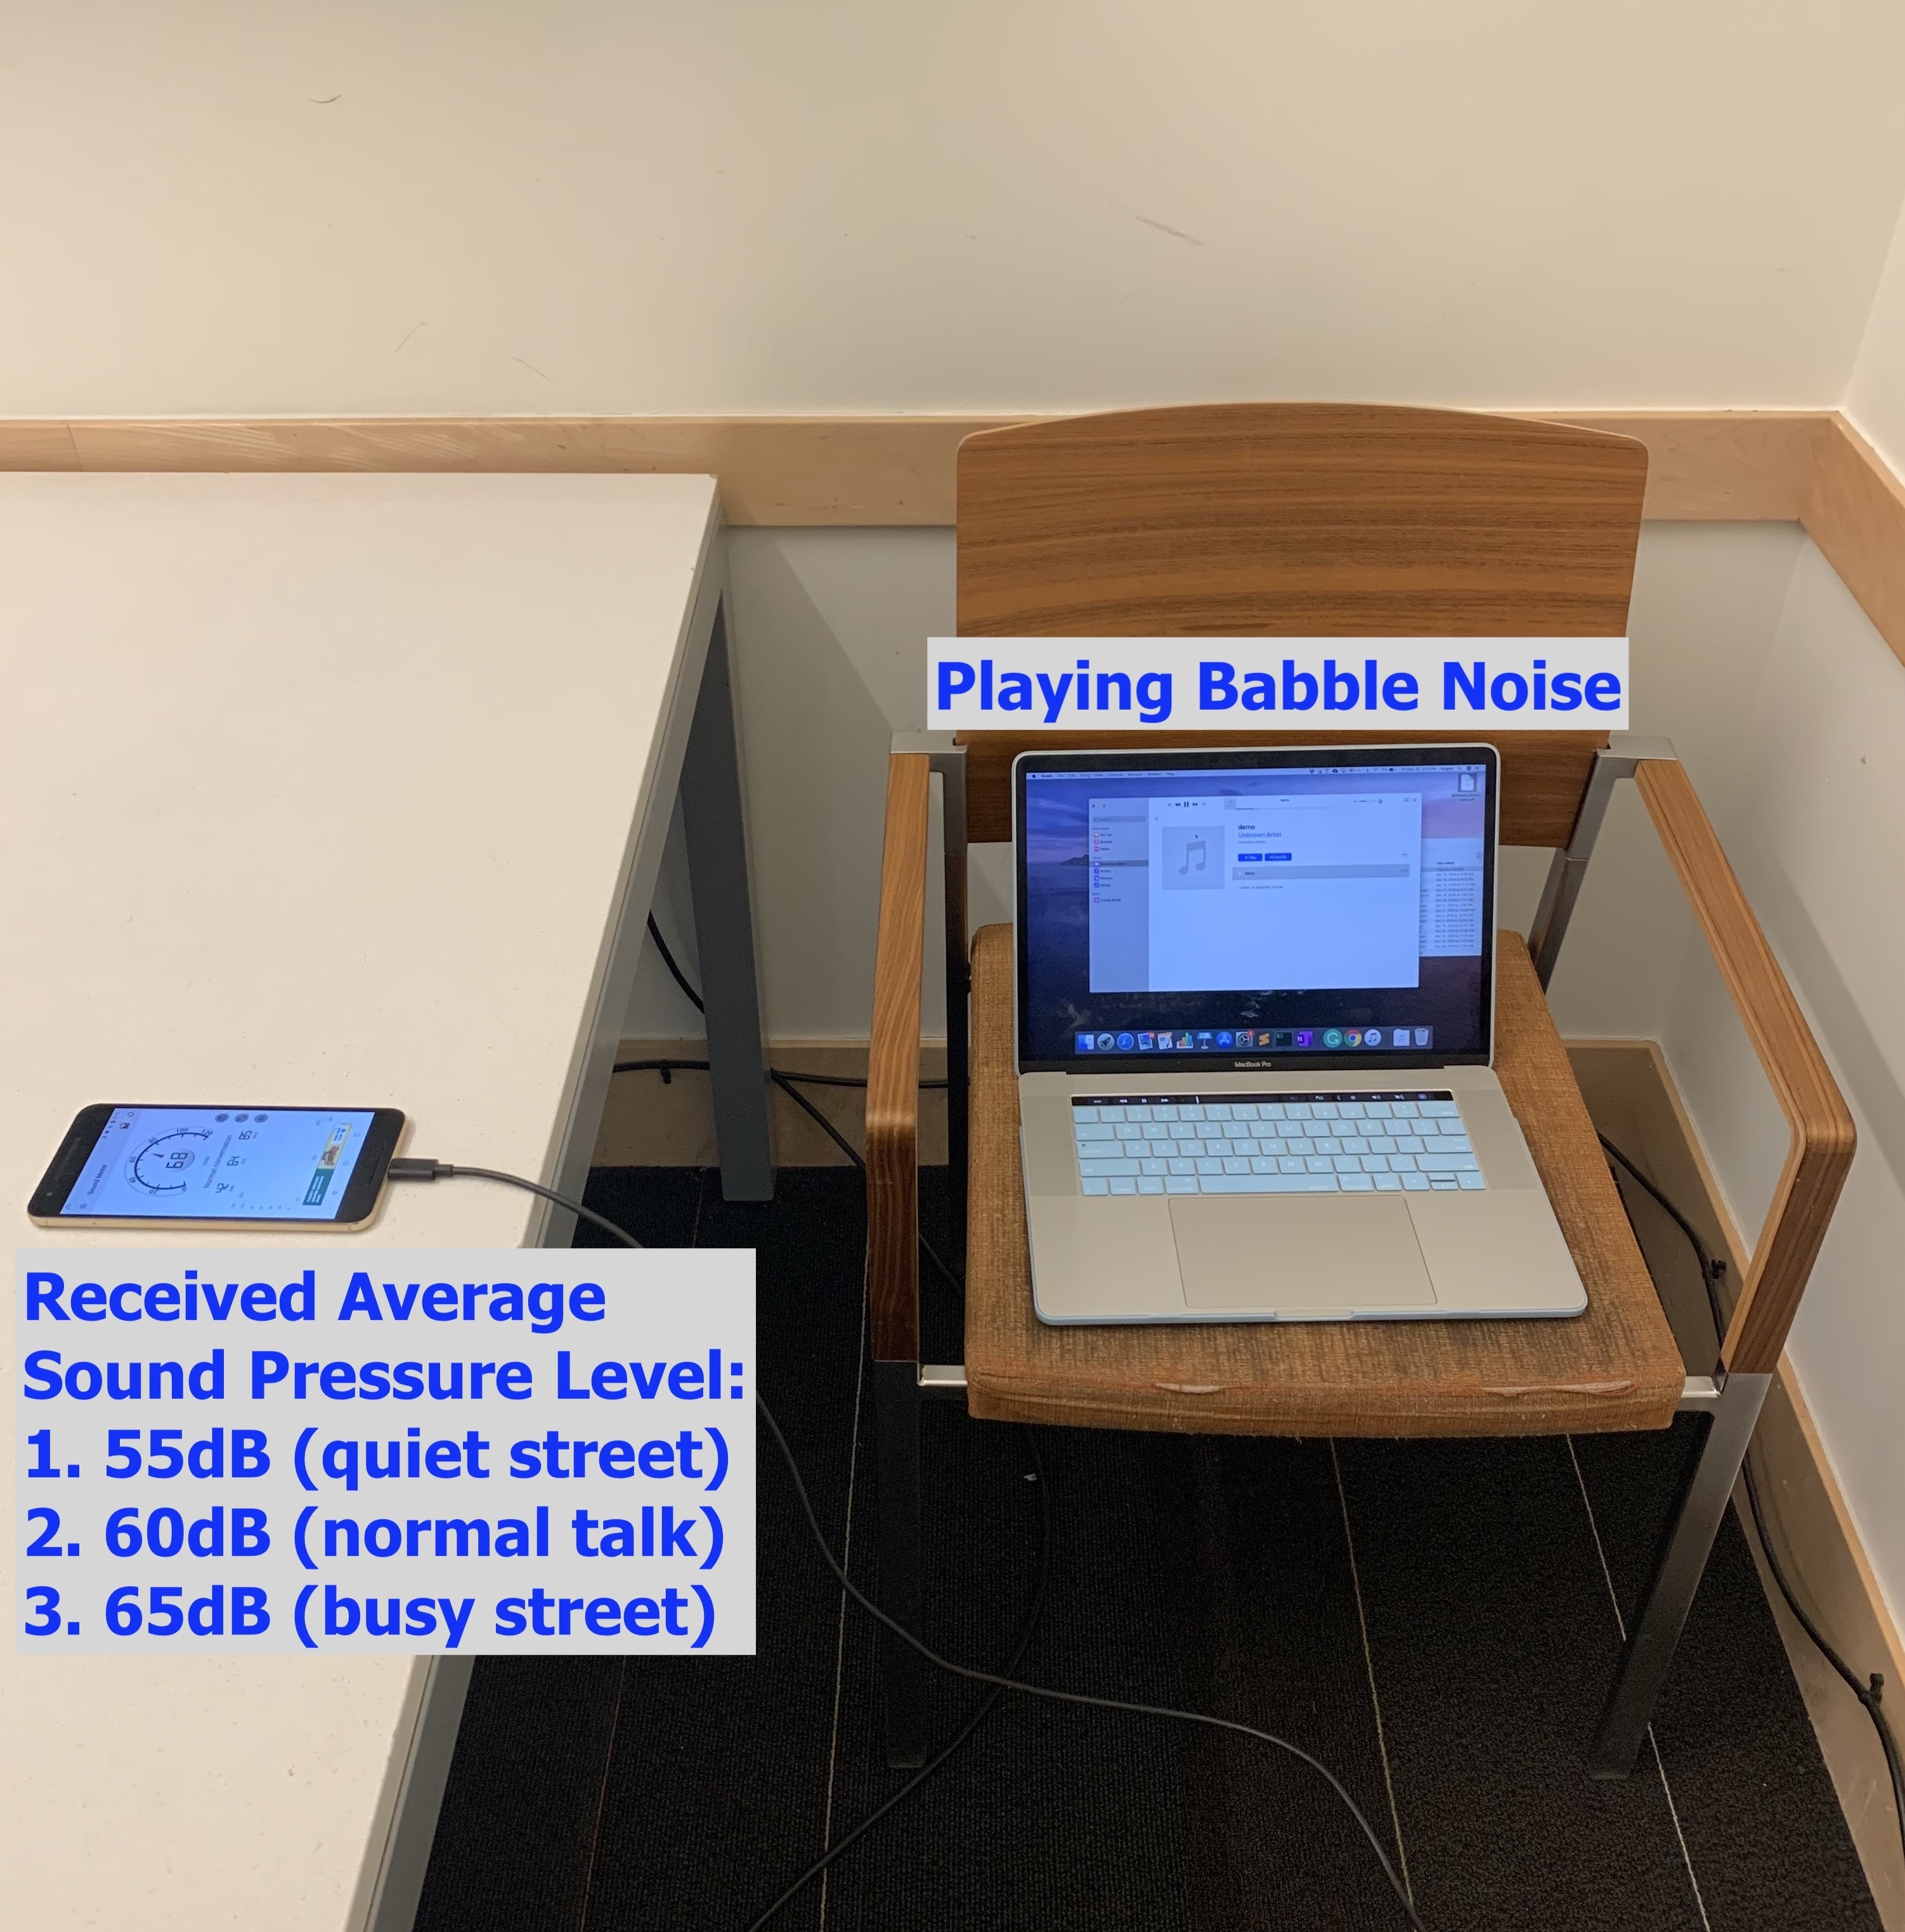
\includegraphics[width=.5\linewidth]{noisetest}
	\caption{Testing Setup.}
	\label{fig:noisetest}
\end{figure}

In this section, we test how background noises like real human talking influence the classification accuracy. When the smartphone speakers are playing sounds, a real person talks 20 cm away from the smartphone, with a similar volume. The result is shown in Figure~\ref{fig:noise}, the overall accuracy for all classes is about 60\%. Since {\systemName} still works in this experiment, it is an evidence that motion sensors are more sensitive to the built-in speakers than other sound sources that transmit signals through the air. 
%
It is worth mentioning that the performance of {\systemName} can be further improved if more training data is added. At this time, all training data are collected in a quiet environment, so directly feeding an input data from a noisy environment decreases the accuracy from 91\% to 60\%. Adding data from various environments, however, is expected to increase the robustness of the system and therefore a future research direction. 



To further test the impact of noises, we use a babble noise file and play the noise with different volumes. We control the sound pressure level received by the target phone to 55dB (quiet urban street), 60dB (normal conversation), and 65 dB (busy street). The results are shown in Figure ~\ref{fig:noisetestresult}.

\begin{landscape}
	\begin{figure}[!h]
		
		\begin{minipage}[c]{.33\linewidth}
			\centering
			\includegraphics[width=\textwidth]{digitDB55CFM}
			\tiny
			\begin{tabular}{lr}
				\toprule
				Accuracy: 88.87\% & \hspace{-.00in} Error Rate: 11.13\% \\
				Precision: 88.87\% & \hspace{-.00in} True Positive Rate: 89.20\% \\
				$F_1$ Score: 0.889 & \hspace{-.00in} True Negative Rate: 98.89\% \\
				False Negative: 10.80\% & \hspace{-.00in} False Positive Rate: 1.11\% \\
				\bottomrule
			\end{tabular}
			\subcaption{Quiet Street (55 dB noise)}
		\end{minipage}
		\begin{minipage}[c]{.33\linewidth}
			\centering
			\includegraphics[width=\textwidth]{digitDB60CFM}
			\tiny
			\begin{tabular}{lr}
				\toprule
				Accuracy: 85.48\% & \hspace{-.00in} Error Rate: 14.52\% \\
				Precision: 85.49\% & \hspace{-.00in} True Positive Rate: 86.16\% \\
				$F_1$ Score: 0.855 & \hspace{-.00in} True Negative Rate: 98.55\% \\
				False Negative: 13.84\% & \hspace{-.00in} False Positive Rate: 1.45\% \\
				\bottomrule
			\end{tabular}
			\subcaption{Normal Conversation (60 dB noise)}
		\end{minipage}
		\begin{minipage}[c]{.33\linewidth}
			\centering
			\includegraphics[width=\textwidth]{digitDB65CFM}
			\tiny
			\begin{tabular}{lr}
				\toprule
				Accuracy: 77.50\% & \hspace{-.00in} Error Rate: 22.50\% \\
				Precision: 77.47\% & \hspace{-.00in} True Positive Rate: 77.61\% \\
				$F_1$ Score: 0.773 & \hspace{-.00in} True Negative Rate: 97.76\% \\
				False Negative: 22.39\% & \hspace{-.00in} False Positive Rate: 2.24\% \\
				\bottomrule
			\end{tabular}
		\subcaption{Noisy Street (65 dB noise)}
		\end{minipage}
		\caption[Impact of Surrounding Environments.]{The Impact of Surrounding Environments: Quiet Street, Normal Conversation, and Noisy Street. Note that the decibel values are the average sound pressure levels received by the smartphone. }
		\label{fig:noisetestresult}
	\end{figure}
\end{landscape}


\subsection{Impact of User Mobility}\label{sec:impact:move}
All previous experiments are conducted when the smartphone is placed on a desk, without being touched or moved during the data collection stage. As illustrated in Figure~\ref{fig:spyphonepreprocess}, user movements are regarded as noises. Fortunately, since user movement is very slow and is unlikely to generate signals as high as 50 Hz. Thus, we can apply a high pass filter to mitigate the noise. In Figure~\ref{fig:newspec}, we see noises are removed after the filter. In this section, we validate the performance of {\systemName} with the presence of user mobility. 

We conduct two experiments: the walking scenario and the driving scenario. The users put the phone in their pockets while playing the sounds using the speakers. The results are shown in Figure~\ref{fig: walkanddrive}. The accuracy for the walking scenario is 83.94\% and that of driving scenario is 73.34\%. The accuracy of the driving scenario is relatively lower because of frequencies of the noises are relatively higher and thus close to the aliasing of human speech.

Moreover, we conduct an experiment in the extreme case that the user holds the phone in the hand and keeps moving it. The results are plotted in Figure~\ref{fig:move}, the average accuracy can still achieve 45\%.

\begin{figure}[!h]
	\centering
	\includegraphics[width=.6\linewidth]{move}
	\caption{Impact of User Mobility.}
	\label{fig:move}
\end{figure}


\begin{landscape}
	\begin{figure}[!h]
		\centering
		\begin{minipage}[c]{.48\linewidth}
			\centering
			\includegraphics[width=\textwidth]{digitWalkCFM}
			\begin{tabular}{lr}
				\toprule
				Accuracy: 83.94\% & \hspace{-.00in} Error Rate: 16.06\% \\
				Precision: 83.94\% & \hspace{-.00in} True Positive Rate: 84.05\% \\
				$F_1$ Score: 0.839 & \hspace{-.00in} True Negative Rate: 98.39\% \\
				False Negative Rate: 15.95\% & \hspace{-.00in} False Positive Rate: 1.61\% \\
				\bottomrule
			\end{tabular}
		\end{minipage}
		\begin{minipage}[c]{.48\linewidth}
			\centering
			\includegraphics[width=\textwidth]{digitDriveCFM}
			\begin{tabular}{lr}
				\toprule
				Accuracy: 73.34\% & \hspace{-.00in} Error Rate: 26.66\% \\
				Precision: 73.34\% & \hspace{-.00in} True Positive Rate: 73.59\% \\
				$F_1$ Score: 0.733 & \hspace{-.00in} True Negative Rate: 97.34\% \\
				False Negative Rate: 26.41\% & \hspace{-.00in} False Positive Rate: 2.66\% \\
				\bottomrule
			\end{tabular}
		\end{minipage}
		\caption[Accuracy in the walking (left) and driving (right) scenario.]{Accuracy in the walking (left) and driving (right) scenario. The machine learning model trained in the stable environment is directly used to predict the testing data collected when user is walking or driving.}
		\label{fig: walkanddrive}
	\end{figure}
\end{landscape}




%


\section{Defenses}
%To defend against an attacker that has only user-level access to the device (an application or a web- site), it might be enough to apply low-pass filtering to the raw samples provided by the gyroscope. Judging by the sampling rate available for Blink and WebKit based browsers, it is enough to pass frequencies in the range 0 – 20 Hz. If this rate is enough for most of the applications, the filtering can be done by the driver or the OS, subvert- ing any attempt to eavesdrop on higher frequencies that reveal information about surrounding sounds. In case a certain application requires an unusually high sampling rate, it should appear in the list of permissions requested by that application, or require an explicit authorization by the user. To defend against attackers who gain root access, this kind of filtering should be performed at the hardware level, not course, it imposes a able to applications.
%Another possible masking. It can be possibly on the case
%being subject to configuration. Of restriction on the sample rate avail-
%solution is some kind of acoustic applied around the sensor only, or
%of the mobile device.

%%TODO take defense?
To defend against the {\attackName} attack, the smartphone user can adopt the hardware-based defenses or the software-based defenses if supported by the smartphone's operating systems.
%\vspace{-.1in}
\subsection{Hardware-based Defenses}
%\textbf{Hardware-based Defenses: }
The easiest way to defend the {\attackName} attack is to not use smartphone's built-in speakers. Instead, a user can use \textit{headphones} or other wireless connected loudspeakers. As long as there is no direct contact between the speakers and the motion sensors, the attack is defended~\cite{anand2018speechless}. In fact, as shown in Section~\ref{sec:impact:volume}, with lower volume setting, the {\attackName} attack can also be largely impeded. Though such hardware-based defenses may cause inconvenience to the user, their security and privacy can be protected.
%Loudspeaker not loud
%newly-released OSchoose to keep the OS version, do not or can not upgrade to the
%Use headphones
%\vspace{-.1in}
\subsection{Software-based Defenses}
%\textbf{Software-based Defenses: }
The software-based defenses are better sensor management by smartphones' operating systems (OS). For example, the OS should treat the permissions to motion sensors as dangerous permissions and require users to grant permissions at installation time. Moreover, the OS should keep monitoring the sensor usage such as when the sensors are used, whether they are used in background, and what sampling rate is required by the application. 


Though there has been some research in designing better sensor management systems~\cite{sikder20176thsense}, the {\attackName} attack may still be a big threat for at least three years. This is because the smartphone users may not or can not upgrade to the 
newly-released OS in a timely manner. 
%For example, more than half the Android devices are still using OS as old as Android Nougat, which was released in 2016\footnote{\scriptsize \url{https://developer.android.com/about/dashboards}}. 
%
Indeed, by the end of May 7, 2019, more than half the Android devices are still using OS released three years ago~\footnote{More than half the Android devices are still using OS as old as Android Nougat, which was released in 2016 according to Android Dashboards (\url{https://developer.android.com/about/dashboards})}. Therefore, three years later, there is a large chance that more than half the devices are still using the OS released so far. Since current Android OS cannot defend the SpyPhone system, those devices are vulnerable to the Man-in-the-Phone attack. However, if smartphone users know the importance of the update and cares about their security and privacy, the adoption speed may increase. Note that there is a huge lag between Google and the manufacturers such as Samsung and Huawei. Even Google release the security updates quickly enough, the manufacturer may release them too late.

%~\cite{onlinedashboards}.
%

\section{Related Work}

\subsection{Inferring  Information From Smartphone Motion Sensors}
%Modern mobile devices such as smartphones are equipped with more and more powerful motion sensors(i.e., accelerometer, gyroscope).
%
In recent years, much attention has been paid to inferring private information  through motion sensors in the literature.
%
A typical side-channel attack is keystrokes inference on smartphones through motion sensors~\cite{owusu2012accessory,miluzzo2012tapprints}. 
%
The general idea of these attacks is that when typing on different locations on a screen, the keystrokes cause distinct vibrations or rotations. 
%
In addition, Wang \emph{et al.}~\cite{wang2015mole} proposed to track the movement of the wrist to infer what the user has typed.
% 
Similarly, a practical attack has been shown in~\cite{wang2016friend}, which infers a user’s personal PIN sequence by exploiting wearable devices.
%
The feasibility of inferring user’s location information using motion sensors instead of GPS data has been shown in~\cite{liang2017location,han2012accomplice}.
%
Bojinov \emph{et al.}~\cite{bojinov2014mobile} demonstrated that motion sensors can be used as device fingerprint to uniquely identify a device. 
%
This motion sensor-based device fingerprint was further utilized by~\cite{das2016tracking} to track a user across multiple visits to websites.
%
In~\cite{lee2018inferring}, Lee \emph{et al.} proposed to use motion sensors to infer users' handwritten patterns.
%
Huang \emph{et al.}~\cite{huang2018breathlive} implemented a reliable liveness detection system called Breathlive, which is based on the inherent correlation between sounds and chest motion caused by deep breathing.
%
Roy \emph{et al.}~\cite{roy2015ripple} demonstrated the possibility of communication through motion sensors by modulating the vibration motor and decoding through accelerometers. 
%
Recent works on activity recognition using motion sensors are presented in~\cite{shoaib2015survey,wang2019deep}.
%
In addition, a detailed survey of works on sensor-based threats for smart devices can be found in~\cite{sikder2018survey, crager2017information}.
%===========================================================
%
Note that we only list related works using smartphone motion sensors, but not works using standalone sensors. This is because smartphone motion sensors can only report readings at a low frequency, but standalone accelerometers or gyroscopes can record signals with frequencies as high as 10 KHz. Some special models of piezoelectric accelerometers can even measure 1~MHz signals.
\subsection{Eavesdropping Sound Signals By Non-Acoustic Sensors}
Recent studies have shown that sound signals can be eavesdropped through non-acoustic sensors instead of microphones.
%
Among these side-channel attacks, MEMS motion sensors are widely used since motion sensors are prone to acoustic signals.
%
Michalevsky \emph{et al.}~\cite{michalevsky2014gyrophone} found that the MEMS gyro sensors are able to pick up air vibrations from sound. 
%
They proposed GyroPhone, a new threat which uses  gyroscope on smartphone to intercept human speech.  
%
Zhang \emph{et al.}~\cite{zhang2015accelword} proposed to utilize accelerometer  for hotword detection to reduce power consumption.
%
In addition, Anand \emph{et al.}~\cite{anand2018speechless} also demonstrated that it is possible to eavesdrop speech signals in certain scenarios by using inertial sensors in a smartphone. 
%
Han \emph{et al.}~\cite{han2017pitchln} proposed to combine multiple signals from non-acoustic sensors to create a higher sample rate signal for speech reconstruction.
%
Hawley \emph{et al.}~\cite{hawley2018visualizing} proposed to use sensors on smartphone to visualize the properties of sound directivity, interference and other acoustical phenomena. 
%
Recently, other techniques have been proposed to eavesdrop sound signals besides motion sensors.
%
Roy \emph{et al.}~\cite{roy2016listening} have shown that the vibration motor  can be used as microphone since the vibrating mass inside the motor responds to air vibrations from nearby sounds.
%
Davis \emph{et al.}~\cite{davis2014visual} used a high speed camera to retrieve digital audio by capturing the vibration of objects near the sound source.
%
Similarly, Fuse \emph{et al.}~\cite{fuse2018sound} found that a better sound can be obtained by trying to recover the sound based on the vibration direction of the object.
%
Kwong \emph{et al.}~\cite{kwonghard} demonstrated that the mechanical components in magnetic hard disk drives can be used to extract and parse human speech with sufficient precision. 


%
%\section{Related Work}
%
%Eaves sound signal using non- acoustic sensor;;
%
%
%Information using motion sensor on smartphone
%acce -> keytroke, pin, ...
%
%
%used to measure angular rotation, across x, y, and z axes.
%Motion sensors have been shown prone to acoustic noise particularly at high frequency and power level in [12], [13], [14], which showed that MEMS gyroscopes are susceptible to high power, high frequency noise that contains frequency components in proximity of the resonating frequency of the gyroscope’s proof mass. This concept of work was further utilized by Son et al. [15] to interfere with the flight control system of a drone using intentional sounds that were produced by a Bluetooth speaker attached to the drones with a sound 
%
%but On smartphones, ~\cite{michalevsky2014gyrophone} are first.
%
%\subsection{Eavasdrop sound signals on smartphones}
%
%visual
%vibration sensor
%
%
%
%
%\subsection{Eavasdrop sound signals using sensors other than microphone}
%
%
%Security of sensor-equipped devices
%
%
%Sensor-based threats [76] on mobile devices have be- come more prevalent than before with the use of dif- ferent sensors in smartphones such as user’s location, keystroke information, etc. Different works [73] have in- vestigated the possibility of these threats and presented different potential threats in recent years. One of the most common threats is keystroke inference in smart- phones. Smartphones use on-screen QWERTY keyboard which has specific position for each button. When a user types in this keyboard, values in smartphone’s motion sensor (i.e., accelerometer and gyroscope) change ac- cordingly [16]. As different keystrokes yield different, but specific values in motion sensors, typing informa- tion on smartphones can be inferred from an unautho- rized sensor such as motion sensor data or motion sen- sor data patterns collected either in the device or from a nearby device can be used to extract users’ input in smartphones [9, 66, 52]. The motion sensor data can be analyzed using different techniques (e.g., machine learning, frequency domain analysis, shared-memory ac- cess, etc.) to improve the accuracy of inference tech- niques such as [12, 53, 81, 46, 58, 47]. Another form of
%keystroke inference threat can be performed by observ- ing only gyroscope data. Smartphones have a feature of creating vibrations while a user types on the touch- pad. The gyroscope is sensitive to this vibrational force and it can be used to distinguish different inputs given by the users on the touchpad [51, 15, 44]. Recently, ICS-CERT also issued an alert for accelerometer-based attacks that can deactivate any device by matching vi- bration frequency of the accelerometer [2, 1, 70]. Light sensor readings also change while a user types on the smartphone; hence, the user input in a smartphone can be inferred by differentiating the light sensor data in nor- mal and typing modes [71]. The light sensor can also be used as a medium to transfer malicious code and trigger message to activate malware [28, 76]. The audio sen- sor of a smartphone can be exploited to launch different malicious attacks (e.g., information leakage, eavesdrop- ping, etc.) on the device. Attackers can infer keystrokes by recording tap noises on touchpad [24], record conver- sation of users [63], transfer malicious code to the device [73, 76], or even replicate voice commands used in voice- enabled different Apps like Siri, Google Voice Search, etc. [21, 39]. Modern smartphone cameras can be used to covertly capture screenshot or video and to infer infor- mation about surroundings or user activities [68, 43, 67]. GPS of a smartphone can be exploited to perform a false data injection attack on smartphones and infer the loca- tion of a specific device [75, 19].
%
%
%
%%\begin{landscape}
	\SingleSpacing
	
	\begin{longtable}{p{3cm}p{6cm}p{6cm}ccc} %p{1.5cm}
		\caption{Related Work on Liveness Detection}
		\label{tab:liveness}
		\\
		
		\toprule
				Authors & Method & Shortcomming & Accuracy & \shortstack{No Extra \\ Devices} &  \shortstack{No Cumbersome \\ User Interaction}  \\
	%			& No User-specific Training\\
		\midrule
		
		\endfirsthead
		
		\normalfont\tablename~\thetable{}~Continued\\
		\toprule
				Authors & Method & Shortcomming & Accuracy & \shortstack{No Extra \\ Devices} &  \shortstack{No Cumbersome \\ User Interaction}  \\
	%			& No User-specific Training\\
		\midrule
		
		\endhead
		
		\bottomrule		
		\endfoot
		
		\endlastfoot
			Girija Chetty and Michael Wagner~\cite{chetty2004automated} & Detecting lip movements using cameras. & Inherits shortcomings of face authentication and introduces high computational overhead. & 99\% & \xmark & \cmark \\
%			& \xmark\\
			Poss et al.~\cite{poss2008biometric} & Using neural tree networks to determine unique aspects of utterances and Hidden Markov Models to classify them. & The accuracy is unkown. & - & \cmark & \cmark 
			\\
%			& \xmark \\
			Wei Shang and Maryhelen Stevenson~\cite{shang2010score} & Testing whether an incoming recording shares the same originating utterance as any of N stored recordings. & Performance is largely based on the pre-stored recordings. & 88.1\%/93.2\% & \cmark & \cmark 
			\\
%			& \xmark \\
			Jes{\'u}s Villalba and Eduardo Lleida~\cite{villalba2011detecting} & Detecting noises and spectrum changes caused by far-field microphone and loudspeakers. & Limits the replay attackers to use far-field microphones. & 91\%-100\% & \cmark & \cmark \\
%			& \cmark \\
			Wang et al.~\cite{wang2011channel} & Detecting channel pattern noise caused by microphone and loudspeakers. & Limits the replay attackers to use low-quality microphones. & 97\% & \cmark & \cmark 
			\\
%			& \cmark \\			
			Aley-Raz et al.~\cite{aley2013device}  & Integrating intra-session voice variation to Nuance VocalPassword~\cite{onlinenuance}. & Requires the user to cumbersomely repeat prompted sentences. & - & \cmark & \xmark 
			\\
%			& \cmark \\
			Zhang et al.~\cite{zhang2016voicelive} & \textbf{VoiceLive}: Measuring the time-difference-of-arrival changes of a sequence of phoneme sounds to the two microphones of the phone. & Requires at least two high-quality microphones in one smartphone. & 99\% & \cmark & \cmark 
			\\
%			& \xmark \\
			Chen et al.~\cite{chen2017you} & Detecting the magnetic field emitted from loudspeakers. & Requires the user to move the smartphone with the predefined trajectory around the sound source. & 100\% & \cmark & \xmark 
			\\
%			& \cmark \\			
			Zhang et al. ~\cite{zhang2017hearing} & \textbf{VoiceGesture}: Leverages Dopler shifts in signals caused by users' articulatory gestures when speaking. & Requires high quality microphones and needs a longer computation time. & 99\% & \cmark & \cmark
			\\
%			 & \xmark \\
			Feng et al.~\cite{feng2017continuous}  & \textbf{VAuth}: Utilizing the instantaneous consistency of the entire signal from the accelerometer and the microphone. & Requires the user to wear high-sampling-rate accelerometers on the facial, throat, or sternum areas. & 97\% & \xmark & \cmark 
			\\
%			& \cmark \\
			Huang et al.~\cite{huang2018breathlive}  & \textbf{BreathLive}: Utilizing chest movement when making deep breaths & The sound is deep breath sound instead of human speech; Stethoscope is needed. & 91\%/94\%/96\% & \xmark & \cmark 
			\\
%			& \xmark \\
			Ment et al.~\cite{meng2018wivo} & \textbf{WiVo}: Using channal state information (CSI) from WiFi signals to detect mouth movement  &  Requires WiFi antennas to collect the CSI info; the distance between antennas and human is short (20cm). & 99\% & \xmark & \cmark
 \\
\bottomrule

\end{longtable}

\end{landscape}

%\begin{landscape}	
%	\begin{table}
%		\centering
%%		\renewcommand{\arraystretch}{1.5}
%%		\caption{Related Work on Liveness Detection}
%%		\label{tab:liveness}
%		\footnotesize
%		\begin{tabular}{p{2.5cm}p{0.5cm}p{4.5cm}p{4.5cm}ccc} %p{1.5cm}
%			\toprule\specialrule{0.5pt}{1.5pt}{\belowrulesep}
%			Authors & Year & Method & Shortcomming & Accuracy & \shortstack{No Extra \\ Devices} &  \shortstack{No Cumbersome \\ User Interaction}  \\
%%			& No User-specific Training\\
%			\midrule
%			Girija Chetty and Michael Wagner~\cite{chetty2004automated} & 2004 & Detecting lip movements using cameras. & Inherits shortcomings of face authentication and introduces high computational overhead. & 99\% & \xmark & \cmark \\
%%			& \xmark\\
%			Poss et al.~\cite{poss2008biometric} & 2008 & Using neural tree networks to determine unique aspects of utterances and Hidden Markov Models to classify them. & The accuracy is unkown. & - & \cmark & \cmark 
%			\\
%%			& \xmark \\
%			Wei Shang and Maryhelen Stevenson~\cite{shang2010score} & 2010 & Testing whether an incoming recording shares the same originating utterance as any of N stored recordings. & Performance is largely based on the pre-stored recordings. & 88.1\%/93.2\% & \cmark & \cmark 
%			\\
%%			& \xmark \\
%			Jes{\'u}s Villalba and Eduardo Lleida~\cite{villalba2011detecting} & 2011 & Detecting noises and spectrum changes caused by far-field microphone and loudspeakers. & Limits the replay attackers to use far-field microphones. & 91\%-100\% & \cmark & \cmark \\
%%			& \cmark \\
%			Wang et al.~\cite{wang2011channel} & 2011 & Detecting channel pattern noise caused by microphone and loudspeakers. & Limits the replay attackers to use low-quality microphones. & 97\% & \cmark & \cmark 
%			\\
%%			& \cmark \\			
%			Aley-Raz et al.~\cite{aley2013device}  & 2013 & Integrating intra-session voice variation to Nuance VocalPassword~\cite{onlinenuance}. & Requires the user to cumbersomely repeat prompted sentences. & - & \cmark & \xmark 
%			\\
%%			& \cmark \\
%			Zhang et al.~\cite{zhang2016voicelive} & 2016 & \textbf{VoiceLive}: Measuring the time-difference-of-arrival changes of a sequence of phoneme sounds to the two microphones of the phone. & Requires at least two high-quality microphones in one smartphone. & 99\% & \cmark & \cmark 
%			\\
%%			& \xmark \\
%			Chen et al.~\cite{chen2017you} & 2017 & Detecting the magnetic field emitted from loudspeakers. & Requires the user to move the smartphone with the predefined trajectory around the sound source. & 100\% & \cmark & \xmark 
%			\\
%%			& \cmark \\			
%			Zhang et al.~\cite{zhang2017hearing} & 2017 & \textbf{VoiceGesture}: Leverages Dopler shifts in signals caused by users' articulatory gestures when speaking. & Requires high quality microphones and needs a longer computation time. & 99\% & \cmark & \cmark
%			\\
%%			 & \xmark \\
%			Feng et al.~\cite{feng2017continuous}  & 2017 & \textbf{VAuth}: Utilizing the instantaneous consistency of the entire signal from the accelerometer and the microphone. & Requires the user to wear high-sampling-rate accelerometers on the facial, throat, or sternum areas. & 97\% & \xmark & \cmark 
%			\\
%%			& \cmark \\
%			Huang et al.~\cite{huang2018breathlive}  & 2018 & \textbf{BreathLive}: Utilizing chest movement when making deep breaths & The sound is deep breath sound instead of human speech; Stethoscope is needed. & 91\%/94\%/96\% & \xmark & \cmark 
%			\\
%%			& \xmark \\
%			Ment et al.~\cite{meng2018wivo} & 2018 & \textbf{WiVo}: Using channal state information (CSI) from WiFi signals to detect mouth movement  &  Requires WiFi antennas to collect the CSI info; the distance between antennas and human is short (20cm). & 99\% & \xmark & \cmark
%			\\
%		\specialrule{0.5pt}{\aboverulesep}{1.5pt}\bottomrule
%		\end{tabular}
%	\end{table}
%\end{landscape}

%Shang et al.~\cite{shang2010score} propose to compare an input voice sample with stored instances of past accesses to detect the voice samples have been seen before by the authentication system. This method, however, cannot work if the attacker records the voice samples during a non-authentication time point. Villalba et al. and Wang et al. suggest that the additional channel noises introduced by the recording and loudspeaker can be used for attack detection~\cite{villalba2011detecting,wang2011channel}.
%These approaches however have limited effec- tiveness in practice. For example, the false acceptance rates of these approaches are as high as 17\%. Chetty and Wagner propose to use video camera to extract lip movements for liveness verification~\cite{chetty2004automated}, whereas Poss et al. combine the techniques of a neural tree network and Hidden Markov Models to improve authentication accuracy~\cite{poss2008biometric}.
%Aley-Raz et al.~\cite{aley2013device} develop a liveness detection system based on ``Intra-session voice variation'', which is integrated into Nuance VocalPassword~\cite{onlinenuance}. In addition to a user-chosen passphrase, it requires a user to repeat one or more random sentences prompted by the system for liveness detection. Such a method however increases the op- eration overhead of the user and is cumbersome due to an explicit user cooperation is required besides the standard authentication process. 
%
%More recently, Chen et al.~\cite{chen2017you} develop a smartphone based liveness detection system by measuring the magnetic field emit- ted from loudspeakers. It however requires the user to speak the passphrase while moving the smartphone with predefined trajectory around the sound source. Moreover, Zhang et al.~\cite{zhang2016voicelive} propose a smarthphone based solution, which measures the time-difference-of-arrival (TDoA) changes of a sequence of phoneme sounds to the two microphones of the phone when a user speaks a passphrase for liveness detection. However, it requires at least two high-accuracy microphones in one smartphone. Zhang et al.~\cite{zhang2017hearing} then propose VoiceGuesture, which leverages a user’s articulatory gestures when speaking a passphrase for liveness detection. However, the calculation overhead is high.
%Feng et al.~\cite{feng2017continuous} present VAuth,  which utilizes the instantaneous consistency of the entire signal from the accelerometer and the microphone.  However, it requires the user to wear a security-assisting device on the facial, throat, or sternum areas. 
%Huang et al.~\cite{huang2018breathlive} present BreathLive, which utilize the inherent correlation between sounds and chest motion caused by deep breathing to realize a reliable liveness detection system. However, it requires special gyroscope and stethoscope. Since it utilizes deep breathing, the sound period is very long (4 sec. for one deep breathing).
%
%In conclusion, the aforementioned approaches either require cumbersome user interaction, or require extra electronic devices, or require long recording time or processing time. Building a good liveness detection component is still an open problem.
%
%Privacy leakage through sensors.
%
%
%information leaks using motion sensors.
%
%
%WALNUT:
%
%Information Leakage
%Information leakage from physical properties, or side-channels, of computing systems are also relevant to analog cybersecurity. Recent studies show that gyroscopes and accelerometers can leak personal information [12]–[13][14][15][16]. Michalevsky et al. show that gyroscopes in smart-phones can be used as a microphone to eavesdrop on conversations [16]. Marquardt et al. demonstrate that smart-phone accelerometers leak enough information to infer keystrokes from a nearby keyboard [12]. Similarly, Owusu and Aviv show smart-phone accelerometer information leakage can be leveraged to infer user touchscreen gestures and key presses to leak passwords and PIN codes to unlock phones [14], [15]. Dey et al. found that process variation in accelerometers yields a unique fingerprint that can uniquely identify a device [13]. These efforts are a reminder that physical attacks on analog sensors render securing data integrity, authentication, and confidentiality between sensors and microprocessors challenging.
%
%~\cite{aaaGoogleSearch,anand2018speechless,crager2017information,davis2014visual,han2017pitchln,jafari2011fast,jafaridictionary,khalifa2016feasibility,khan2018firearm,maruri2018v,matic2012speech,michalevsky2014gyrophone,michalevsky2014gyrophone,roy2016listening,sikder20176thsense,song2016my,wei2015acoustic,welsh2017smartphone,zhang2015accelword}
%
\section{conclusion}

Self demodulation and acoustic attenuation can be used to build {\shortname}, a spoof-proof voice authentication system. When a user speaks with the smartphone placed on his throat, his voice not only influences the microphone readings, but also affects the accelerometer and gyroscopes. By adopting a sequence-to-sequence long short-term memory network, syllable separation, and majority voting, \shortname~can defend against 3 different types of attacks with 90.43\% defend rate and a 92.98\% acceptance rate for legitimate users.




\begin{landscape}
	\begin{figure}[h]
		\centering
		\begin{minipage}{.48\linewidth}
			\includegraphics[width=\linewidth]{movoUserBefore}
			\subcaption{Without Majority Voting}\label{fig:usermata}
			\vspace{.05in}
		\end{minipage}
		\begin{minipage}{.48\linewidth}
			\includegraphics[width=\linewidth]{movoUserAfter}
			\subcaption{With Majority Voting}\label{fig:usermatb}
			\vspace{.05in}
		\end{minipage}
		\caption{Confusion Matrix of Matching Motion Data to Different Users.}
		\label{fig:usermat}
	\end{figure}
\end{landscape}
